\documentclass{vkr}
\usepackage[english, russian]{babel} % переносы
\usepackage{graphicx} % для вставки картинок
\graphicspath{{images/}} % путь к изображениям
\usepackage[hidelinks]{hyperref}
\usepackage{enumitem}
\renewcommand{\labelitemi}{\textbullet}
\usepackage{float} % определяет метод H для рисунка с переносом на следующую страницу, ели не помещается
\usepackage{pdflscape}
\addto{\captionsrussian}{\renewcommand{\refname}{СПИСОК ИСПОЛЬЗОВАННЫХ ИСТОЧНИКОВ}}
\usepackage{xltabular} % для вставки таблиц
\usepackage{makecell}
\renewcommand\theadfont{} % шрифт в /thead
\usepackage{array} % для определения новых типов столбцов таблиц
\newcolumntype{T}{>{\centering\arraybackslash}X} % новый тип столбца T - автоматическая ширина столбца с выравниванием по центру
\newcolumntype{R}{>{\raggedleft\arraybackslash}X} % новый тип столбца R - автоматическая ширина столбца с выравниванием по правому краю
\newcolumntype{C}[1]{>{\centering\let\newline\\\arraybackslash\hspace{0pt}}m{#1}} % новый тип столбца C - фиксированная ширина столбца с выравниванием по центру
\newcolumntype{r}[1]{>{\raggedleft\arraybackslash}p{#1}} % новый тип столбца r - фиксированная ширина столбца с выравниванием по правому краю
\newcommand{\centrow}{\centering\arraybackslash} % командой \centrow можно центрировать одну ячейку (заголовок) в столбце типа X или p, оставив в оcтальных ячейках другой тип выравнивания
\newcommand{\finishhead}{\endhead\hline\endlastfoot}
\newcommand{\continuecaption}[1]{\captionsetup{labelformat=empty} \caption[]{#1}\\ \hline }
\usepackage{etoolbox}
\AtBeginEnvironment{xltabular}{\refstepcounter{tablecnt}} % подсчет таблиц xltabular, обычные таблицы подсчитываются в классе

\usepackage[tableposition=top]{caption} % подпись таблицы вверху
\captionsetup{strut=off}
\setlength{\intextsep}{0pt} % Vertical space above & below [h] floats
\setlength{\textfloatsep}{0pt} % Vertical space below (above) [t] ([b]) floats
\DeclareCaptionLabelFormat{gostfigure}{Рисунок #2} %подпись рисунка
\DeclareCaptionLabelFormat{gosttable}{Таблица #2} %подпись таблицы
\DeclareCaptionLabelSeparator{gost}{~--~} %разделитель в рисунках и таблицах
\captionsetup{labelsep=gost}
\captionsetup[figure]{aboveskip=10pt,belowskip=4mm,justification=centering,labelformat=gostfigure} % настройка подписи рисунка
\captionsetup[table]{font={stretch=1.41},skip=0pt,belowskip=0pt,aboveskip=8.5pt,singlelinecheck=off,labelformat=gosttable} % настройка подписи таблицы

\setlength{\LTpre}{8mm} % отступ сверху таблицы
\setlength{\LTpost}{6mm} % отступ снизу таблицы

\usepackage{enumitem}
\setlist{nolistsep,wide=\parindent,itemindent=*} % отступы вокруг списков, выравнивание с учетом разделителя

\usepackage{color} %% это для отображения цвета в коде
\usepackage{listings} %% листинги кода
\setmonofont[Scale=0.7]{Verdana} % моноширный шрифт для листинга

\definecolor{codegreen}{rgb}{0,0.6,0}
\definecolor{codegray}{rgb}{0.5,0.5,0.5}
\definecolor{codepurple}{rgb}{0.58,0,0.82}

\lstset{ %
language=C,                 % выбор языка для подсветки (здесь это С)
numbers=left,               % где поставить нумерацию строк (слева\справа)
numberstyle=\tiny,           % размер шрифта для номеров строк
stepnumber=1,                   % размер шага между двумя номерами строк
numbersep=5pt,                % как далеко отстоят номера строк от подсвечиваемого кода
commentstyle=\color{codegreen},
keywordstyle=\color{magenta},
numberstyle=\tiny\color{codegray},
stringstyle=\color{codepurple},
basicstyle=\linespread{0.95}\ttfamily,
backgroundcolor=\color{white}, % цвет фона подсветки - используем \usepackage{color}
showspaces=false,            % показывать или нет пробелы специальными отступами
showstringspaces=false,      % показывать или нет пробелы в строках
showtabs=false,             % показывать или нет табуляцию в строках
frame=single,              % рисовать рамку вокруг кода
tabsize=2,                 % размер табуляции по умолчанию равен 2 пробелам
captionpos=t,              % позиция заголовка вверху [t] или внизу [b] 
breaklines=true,           % автоматически переносить строки (да\нет)
breakatwhitespace=false, % переносить строки только если есть пробел
escapeinside={\%*}{*)}   % если нужно добавить комментарии в коде
}

\makeatletter % чтобы допускались русские комментарии в листингах
\lst@InputCatcodes
\def\lst@DefEC{%
 \lst@CCECUse \lst@ProcessLetter
  ^^80^^81^^82^^83^^84^^85^^86^^87^^88^^89^^8a^^8b^^8c^^8d^^8e^^8f%
  ^^90^^91^^92^^93^^94^^95^^96^^97^^98^^99^^9a^^9b^^9c^^9d^^9e^^9f%
  ^^a0^^a1^^a2^^a3^^a4^^a5^^a6^^a7^^a8^^a9^^aa^^ab^^ac^^ad^^ae^^af%
  ^^b0^^b1^^b2^^b3^^b4^^b5^^b6^^b7^^b8^^b9^^ba^^bb^^bc^^bd^^be^^bf%
  ^^c0^^c1^^c2^^c3^^c4^^c5^^c6^^c7^^c8^^c9^^ca^^cb^^cc^^cd^^ce^^cf%
  ^^d0^^d1^^d2^^d3^^d4^^d5^^d6^^d7^^d8^^d9^^da^^db^^dc^^dd^^de^^df%
  ^^e0^^e1^^e2^^e3^^e4^^e5^^e6^^e7^^e8^^e9^^ea^^eb^^ec^^ed^^ee^^ef%
  ^^f0^^f1^^f2^^f3^^f4^^f5^^f6^^f7^^f8^^f9^^fa^^fb^^fc^^fd^^fe^^ff%
  ^^^^20ac^^^^0153^^^^0152%
  % Basic Cyrillic alphabet coverage
  ^^^^0410^^^^0411^^^^0412^^^^0413^^^^0414^^^^0415^^^^0416^^^^0417%
  ^^^^0418^^^^0419^^^^041a^^^^041b^^^^041c^^^^041d^^^^041e^^^^041f%
  ^^^^0420^^^^0421^^^^0422^^^^0423^^^^0424^^^^0425^^^^0426^^^^0427%
  ^^^^0428^^^^0429^^^^042a^^^^042b^^^^042c^^^^042d^^^^042e^^^^042f%
  ^^^^0430^^^^0431^^^^0432^^^^0433^^^^0434^^^^0435^^^^0436^^^^0437%
  ^^^^0438^^^^0439^^^^043a^^^^043b^^^^043c^^^^043d^^^^043e^^^^043f%
  ^^^^0440^^^^0441^^^^0442^^^^0443^^^^0444^^^^0445^^^^0446^^^^0447%
  ^^^^0448^^^^0449^^^^044a^^^^044b^^^^044c^^^^044d^^^^044e^^^^044f%
  ^^^^0401^^^^0451%
  %%%
  ^^00}
\lst@RestoreCatcodes
\makeatother


% Режим шаблона (должен быть включен один из трех)
% \ВКРtrue
\Практикаtrue
%\Курсоваяtrue

\newcommand{\Дисциплина}{<<Проектирование и архитектура программных систем>>} % для курсовой
\newcommand{\КодСпециальности}{09.03.04} % Курсовая
\newcommand{\Специальность}{Программная инженерия} % Курсовая
\newcommand{\Тема}{Разработка веб-платформы для автоматизации бизнес-процессов управления персоналом компании} % ВКР Курсовая
\newcommand{\ТемаВтораяСтрока}{1С-Битрикс}
\newcommand{\ГдеПроводитсяПрактика}{ООО <<Предприятие ВТИ-Сервис>>} % для практики
\newcommand{\РуководительПрактПредпр}{Куркина А. В.} % для практики
\newcommand{\ДолжнРуководительПрактПредпр}{директор} % для практики
\newcommand{\РуководительПрактУнивер}{Чаплыгин А. А.} % для практики
\newcommand{\ДолжнРуководительПрактУнивер}{к.т.н. доцент} % для практики
\newcommand{\Автор}{И. А. Седых}
\newcommand{\АвторРод}{Седых И.А.}
\newcommand{\АвторПолностьюРод}{Седых Ивана Александровича} % для практики
\newcommand{\Шифр}{21-06-0028}
\newcommand{\Курс}{4 } % для практики
\newcommand{\Группа}{ПО-11б}
\newcommand{\Руководитель}{А. А. Чаплыгин} % для ВКР и курсовой
\newcommand{\Нормоконтроль}{А. А. Чаплыгин} % для ВКР
\newcommand{\ЗавКаф}{А. В. Малышев} % для ВКР
\newcommand{\ДатаПриказа}{«07» апреля 2023~г.} % для ВКР
\newcommand{\НомерПриказа}{1505-с} % для ВКР
\newcommand{\СрокПредоставления}{«13» июня 2023~г.} % для ВКР, курсового

\begin{document}
\maketitle
\ifПрактика{}\else{
   \newpage
\begin{center}
\large\textbf{Минобрнауки России}

\large\textbf{Юго-Западный государственный университет}
\vskip 1em
\normalsize{Кафедра программной инженерии}
\vskip 1em
\ifВКР{
        \begin{flushright}
        \begin{tabular}{p{.4\textwidth}}
        \centrow УТВЕРЖДАЮ: \\
        \centrow Заведующий кафедрой \\
        \hrulefill \\
        \setarstrut{\footnotesize}
        \centrow\footnotesize{(подпись, инициалы, фамилия)}\\
        \restorearstrut
        «\underline{\hspace{1cm}}»\label{{\tiny }}
        \underline{\hspace{3cm}}
        20\underline{\hspace{1cm}} г.\\
        \end{tabular}
        \end{flushright}
        }\fi
\end{center}
\vspace{1em}
  \begin{center}
  \large
\ifВКР{
ЗАДАНИЕ НА ВЫПУСКНУЮ КВАЛИФИКАЦИОННУЮ РАБОТУ
  ПО ПРОГРАММЕ БАКАЛАВРИАТА}
  \else
ЗАДАНИЕ НА КУРСОВУЮ РАБОТУ (ПРОЕКТ)
\fi
\normalsize
  \end{center}
\vspace{1em}
{\parindent0pt
  Студента \АвторРод, шифр\ \Шифр, группа \Группа
  
1. Тема «\Тема\ \ТемаВтораяСтрока»
\ifВКР{
утверждена приказом ректора ЮЗГУ от \ДатаПриказа\ № \НомерПриказа
}\fi.

2. Срок предоставления работы к защите \СрокПредоставления

3. Исходные данные для создания программной системы:

3.1. Перечень решаемых задач:}

\renewcommand\labelenumi{\theenumi)}

\begin{enumerate}
\item проанализировать IT-инфраструктуру предприятия;
\item  разработать концептуальную модель системы управления IT-ин\-фра\-струк\-турой предприятия на основе подхода к управлению и организации ИТ-услуг ITSM;
\item спроектировать программную систему управления IT-ин\-фра\-струк\-турой предприятия;
\item сконструировать и протестировать программную систему управления IT-инфраструктурой предприятия.
\end{enumerate}

{\parindent0pt
  3.2. Входные данные и требуемые результаты для программы:}

\begin{enumerate}
\item Входными данными для программной системы являются: данные
справочников комплектующих, конфигураций, ПО, критериев качества SLA,
ИТ-услуг, департаментов компании; технические данные ИТ-ресурсов; данные входящих заявок на ИТ-ресурсы; данные запросов поставщикам на комплектующие.
\item Выходными данными для программной системы являются: сформированные заявки на обслуживание ИТ-ресурсов; сформированные запросы на
закупку комплектующих; сведения о выполненных работах по заявкам; статусы заявок; выходные отчеты (инфографика) – по качеству услуг, по состоянию ИТ-ресурсов, по деятельности ИТ-отдела, по стоимости обслуживания
ИТ-ресурсов, воронка заявок.
\end{enumerate}

{\parindent0pt

  4. Содержание работы (по разделам):
  
  4.1. Введение.
  
  4.1. Анализ предметной области.
  
4.2. Техническое задание: основание для разработки, назначение разработки,
требования к программной системе, требования к оформлению документации.

4.3. Технический проект: общие сведения о программной системе, проект
данных программной системы, проектирование архитектуры программной системы, проектирование пользовательского интерфейса программной системы.

4.4. Рабочий проект: спецификация компонентов и классов программной системы, тестирование программной системы, сборка компонентов программной системы.

4.5. Заключение.

4.6. Список использованных источников.

5. Перечень графического материала:

\списокПлакатов

\vskip 2em
\begin{tabular}{p{6.8cm}C{3.8cm}C{4.8cm}}
Руководитель \ifВКР{ВКР}\else работы (проекта) \fi & \lhrulefill{\fill} & \fillcenter\Руководитель\\
\setarstrut{\footnotesize}
& \footnotesize{(подпись, дата)} & \footnotesize{(инициалы, фамилия)}\\
\restorearstrut
Задание принял к исполнению & \lhrulefill{\fill} & \fillcenter\Автор\\
\setarstrut{\footnotesize}
& \footnotesize{(подпись, дата)} & \footnotesize{(инициалы, фамилия)}\\
\restorearstrut
\end{tabular}
}

\renewcommand\labelenumi{\theenumi.}

   \abstract{РЕФЕРАТ}

Объем работы равен \formbytotal{lastpage}{страниц}{е}{ам}{ам}. Работа содержит \formbytotal{figurecnt}{иллюстраци}{ю}{и}{й}, \formbytotal{tablecnt}{таблиц}{у}{ы}{}, \arabic{bibcount} библиографических источников и \formbytotal{числоПлакатов}{лист}{}{а}{ов} графического материала. Количество приложений – 2. Графический материал представлен в приложении А. Фрагменты исходного кода представлены в приложении Б.

Перечень ключевых слов: обучающая платформа, веб-приложение, Django, мультиязычность, CKEditor, AOS, JavaScript, курсы, уроки, тесты, достижения, база данных, ORM, шаблонизатор, аутентификация, иностранные студенты, самостоятельная работа, программирование, прогресс, аналитика, веб-форма, интерактивность, информационные технологии, контент-редактор, администратор, пользователь, веб-интерфейс.

Объектом разработки является веб-приложение -- обучающая платформа, предназначенная для компьютерной поддержки самостоятельной работы иностранных студентов при изучении языка программирования JavaScript, с мультиязычным интерфейсом и интерактивными инструментами для обучения.

Целью выпускной квалификационной работы является создание удобной и функциональной платформы для самостоятельного изучения языка программирования JavaScript иностранными студентами, обеспечивающей доступ к образовательным материалам, тестированию и отслеживанию прогресса через мультиязычный интерфейс, способствующий повышению вовлечённости и эффективности обучения.

В процессе создания платформы были выделены основные сущности (курсы, уроки, тесты, вопросы, ответы, достижения, прогресс студентов) путем проектирования моделей данных, использованы классы и методы Django для обеспечения работы с сущностями, связанными с обучением JavaScript, а также корректного функционирования веб-приложения, разработаны разделы для управления курсами, уроками, тестами по JavaScript, аналитикой прогресса и достижений, реализованы интерактивные элементы с использованием CKEditor для редактирования учебного контента и AOS для анимации интерфейса.

При разработке платформы использовался фреймворк Django с интегрированными библиотеками для аутентификации, шаблонизации, обработки форм и мультиязычности, а также CKEditor и AOS для обеспечения интерактивности и удобства работы с учебным контентом.

Разработанная платформа была успешно протестирована и внедрена в систему обучения.

\selectlanguage{english}
\abstract{ABSTRACT}
  
The volume of work is \formbytotal{lastpage}{page}{}{s}{s}. The work contains \formbytotal{figurecnt}{illustration}{}{s}{s}, \formbytotal{tablecnt}{table}{}{s}{s}, \arabic{bibcount} bibliographic sources and \formbytotal{числоПлакатов}{sheet}{}{s}{s} of graphic material. The number of applications is 2. The graphic material is presented in annex A. The layout of the site, including the connection of components, is presented in annex B.

List of keywords: learning platform, web application, Django, multilingualism, CKEditor, AOS, JavaScript, courses, lessons, tests, achievements, database, ORM, templating, authentication, international students, independent work, programming, progress, analytics, web form, interactivity, information technology, content editor, administrator, user, web interface.

The object of development is a web application -- a learning platform designed for computer support of international students' independent work when learning the JavaScript programming language, with a multi-lingual interface and interactive learning tools.

The aim of the final qualification work is to create a convenient and functional platform for independent learning of JavaScript programming language by foreign students, providing access to educational materials, testing and progress tracking through a multi-lingual interface, which contributes to increased involvement and efficiency of learning.

In the process of creating the platform, the main entities (courses, lessons, tests, questions, answers, achievements, students' progress) were identified by designing data models, Django classes and methods were used to ensure work with entities related to JavaScript learning and correct functioning of the web application, sections for managing courses, lessons, JavaScript tests, progress and achievements analytics were developed, interactive elements were implemented using CKEditor for editing learning content and AOS for interface animation.

The Django framework with integrated libraries for authentication, templating, form processing and multi-language, as well as CKEditor and AOS for interactivity and usability of the learning content were used in the development of the platform.

The developed platform was successfully tested and implemented in the training system.
\selectlanguage{russian}
}\fi
\tableofcontents
\section*{ОБОЗНАЧЕНИЯ И СОКРАЩЕНИЯ}

БД -- база данных.

ИС -- информационная система.

ИТ -- информационные технологии. 

КТС -- комплекс технических средств.

ОМТС -- отдел материально-технического снабжения. 

ПО -- программное обеспечение.

РП -- рабочий проект.

СУБД -- система управления базами данных.

ТЗ -- техническое задание.

ТП -- технический проект.

UML (Unified Modelling Language) -- язык графического описания для объектного моделирования в области разработки программного обеспечения.

\ifПрактика{}\else{\section*{ВВЕДЕНИЕ}
\addcontentsline{toc}{section}{ВВЕДЕНИЕ}

Современные информационные технологии играют ключевую роль в образовательном процессе, обеспечивая доступ к учебным материалам и поддерживая самостоятельное обучение. Обучающие платформы становятся важным инструментом для изучения программирования, особенно для иностранных студентов, которым требуется гибкий и доступный формат обучения с учетом языковых особенностей. Язык программирования JavaScript является одним из наиболее востребованных в веб-разработке благодаря своей универсальности и широкому применению в создании интерактивных веб-приложений. Разработка специализированных веб-приложений для обучения JavaScript позволяет эффективно организовать процесс самостоятельной работы студентов, предоставляя структурированные курсы, интерактивные тесты и отслеживание прогресса.

Веб-приложение, ориентированное на иностранных студентов, предполагает использование мультиязычного интерфейса и интерактивных инструментов, таких как редакторы контента и анимации, для повышения вовлеченности и удобства обучения. Такие платформы позволяют студентам изучать JavaScript в удобном темпе, а преподавателям — эффективно управлять образовательным контентом и отслеживать результаты.

Создание веб-приложения для обучения программированию способствует не только повышению квалификации студентов, но и расширению доступности образования для международной аудитории. Платформа становится инструментом, который объединяет образовательные ресурсы, тестирование и аналитику в единой цифровой среде, упрощая процесс обучения и делая его более интерактивным.

Цель настоящей работы – разработка веб-приложения для компьютерной поддержки самостоятельной работы иностранных студентов при изучении языка программирования JavaScript, обеспечивающего доступ к образовательным материалам, тестированию и отслеживанию прогресса через мультиязычный интерфейс для повышения эффективности обучения. Для достижения поставленной цели необходимо решить следующие задачи:
\begin{itemize}
	\item провести анализ предметной области и требований к обучающим платформам для иностранных студентов;
	\item разработать концептуальную модель веб-приложения для обучения JavaScript;
	\item спроектировать веб-приложение с учетом мультиязычности и интерактивности;
	\item реализовать веб-приложение средствами современных веб-технологий.
\end{itemize}

\emph{Структура и объем работы.} Отчет состоит из введения, 4 разделов основной части, заключения, списка использованных источников, 2 приложений. Текст выпускной квалификационной работы равен \formbytotal{lastpage}{страниц}{е}{ам}{ам}.

\emph{Во введении} сформулирована цель работы, поставлены задачи разработки, описана структура работы, приведено краткое содержание каждого из разделов.

\emph{В первом разделе} на стадии анализа предметной области приводится сбор информации о требованиях к обучающим платформam's для иностранных студентов, изучающих JavaScript, и особенностях организации самостоятельной работы.

\emph{Во втором разделе} на стадии технического задания приводятся требования к разрабатываемому веб-приложению, включая поддержку мультиязычности и интерактивных элементов.

\emph{В третьем разделе} на стадии технического проектирования представлены проектные решения для веб-приложения, включая модели данных и структуру интерфейса.

\emph{В четвертом разделе} приводится список классов и их методов, использованных при разработке платформы, а также результаты тестирования разработанного веб-приложения.

В заключении излагаются основные результаты работы, полученные в ходе разработки.

В приложении А представлен графический материал.
В приложении Б представлены фрагменты исходного кода. 
}\fi
\section{Анализ предметной области}
\subsection{Принцип работы программно-информационной системы управления обучением}

В условиях глобализации образовательных процессов и роста числа иностранных студентов, изучающих программирование, возникает потребность в специализированных программных системах, обеспечивающих поддержку самостоятельного обучения. Согласно международным стандартам качества образования, такие системы должны предоставлять доступ к учебным материалам, автоматизировать проверку знаний и учитывать языковые особенности пользователей. Веб-приложение для компьютерной поддержки самостоятельной работы иностранных студентов при изучении языка программирования JavaScript позволяет автоматизировать ключевые процессы обучения. Рассмотрим основные из них:

\subsubsection{Управление курсами}
После создания курса преподавателем через интерфейс системы, он становится доступным для записи студентов. Курс включает уроки и тесты, которые автоматически отображаются в панели студента. Студент может записаться на курс, просмотреть его содержание и начать обучение. Система фиксирует прогресс студента, а данные о записи передаются в базу данных SQLite для дальнейшей аналитики.

\subsubsection{Управление уроками}
Преподаватели могут добавлять уроки через форму, редактировать их и сортировать с помощью Sortable.js. Каждый урок содержит описание, материалы и тесты. Система автоматически проверяет доступность урока для студента: доступ к следующему уроку открывается только после выполнения теста предыдущего урока. Уроки поддерживают локализацию через Django i18n, что позволяет иностранным студентам выбирать язык интерфейса.


\subsubsection{Управление тестами}
Система автоматизирует создание и управление тестами. Преподаватель может добавлять вопросы и ответы, указывать правильные варианты и проходной балл. Студенты проходят тесты через интерфейс урока, а система автоматически подсчитывает баллы и фиксирует результаты. Для иностранных студентов предусмотрена локализация вопросов и ответов, что упрощает процесс тестирования.

\subsubsection{Аналитика и результаты}
Для анализа успеваемости студентов система предоставляет модуль управления результатами. Преподаватель может просматривать результаты тестов, включая средний балл, максимальный и минимальный, а также удалять их при необходимости. Студенты получают доступ к своим результатам через панель, что позволяет отслеживать прогресс. Данные хранятся в базе SQLite и доступны для аналитики. 

\subsubsection{Поддержка пользователей} 
Система включает модуль управления пользователями, который поддерживает регистрацию студентов и преподавателей. Для иностранных студентов предусмотрена смена языка интерфейса через Django i18n, что обеспечивает комфортное использование. Также система фиксирует роли пользователей и ограничивает доступ к функционалу через декораторы.


\subsection{Компоненты программно-информационной системы управления обучением}
Программно-информационная система управления обучением представляет собой комплекс взаимодействующих программных модулей, аппаратных средств и технологий, предназначенных для хранения, обработки и предоставления образовательного контента. Важным условием функционирования системы является наличие интернет-соединения, обеспечивающего взаимодействие между клиентской и серверной частями. Для обеспечения безопасности данных используется аутентификация через Django contrib.auth, а также защита маршрутов (@loginrequired). На рисунке ~\ref{system:image} представлена схема взаимодействия компонентов системы управления обучением, а также способы их взаимодействия. 

\begin{figure}[ht]
	\centering
	\center{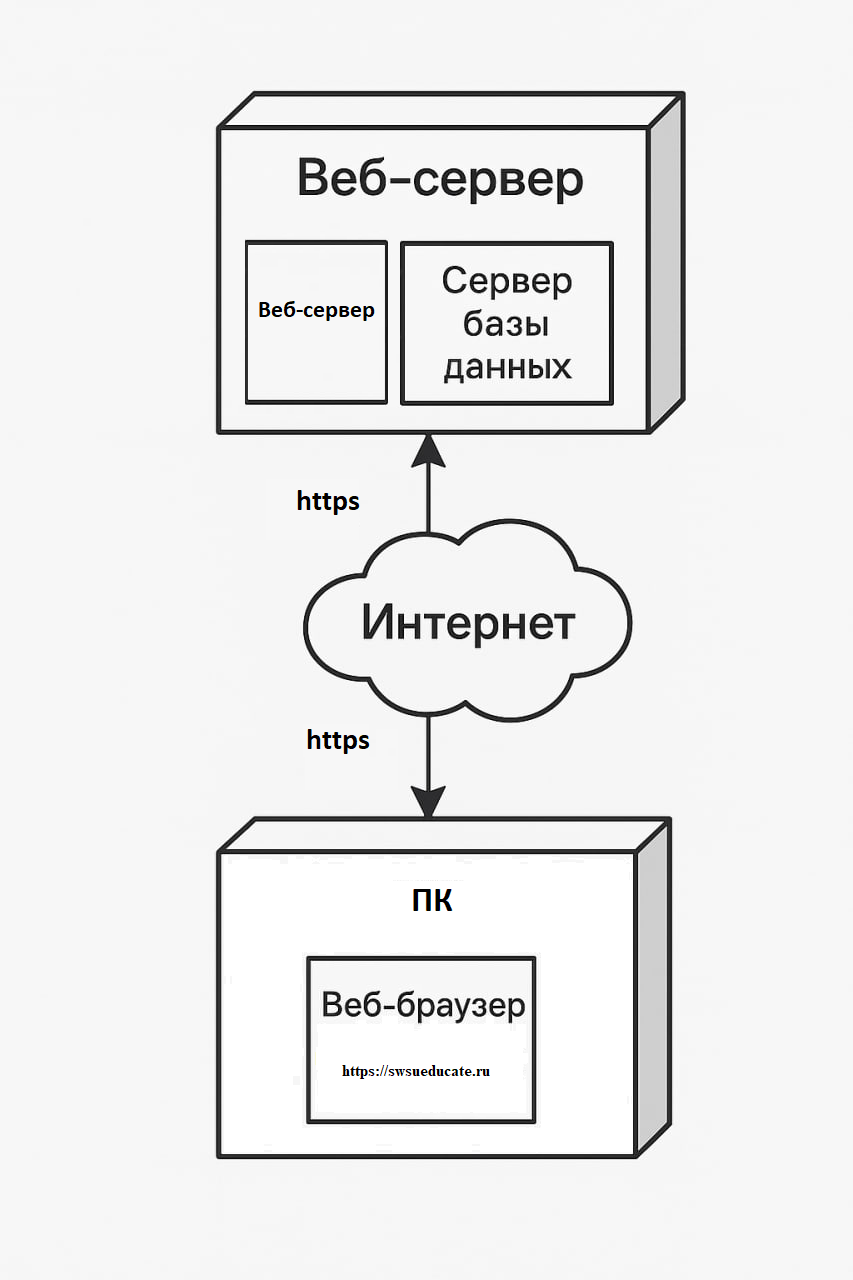
\includegraphics[width=0.57\linewidth]{images/диаграмма2}} 
	\caption{Схема взаимодействия компонентов системы управления обучением}
	\label{system:image}
\end{figure}


\subsection{Отчёты успеваемости}
Одной из причин использования веб-приложения в образовательных целях является удобство формирования отчётов об успеваемости. В системе предусмотрен модуль аналитики, в котором представлена статистическая информация для таких категорий, как прогресс студентов, результаты тестов и активность пользователей. Рассмотрим ключевой отчёт:

\subsubsection{Отчёт по результатам тестов}
Отчёт по результатам тестов представляет собой документ, фиксирующий итоги выполнения тестов студентами за определённый период. Он формирует данные о баллах на момент начала и завершения теста, сведения об общем количестве попыток (attemptnumber), информацию о проходном балле, а также статистику: средний, максимальный и минимальный балл. Пример отчёта представлен на рисунке. 

\begin{figure}[ht]
	\centering
	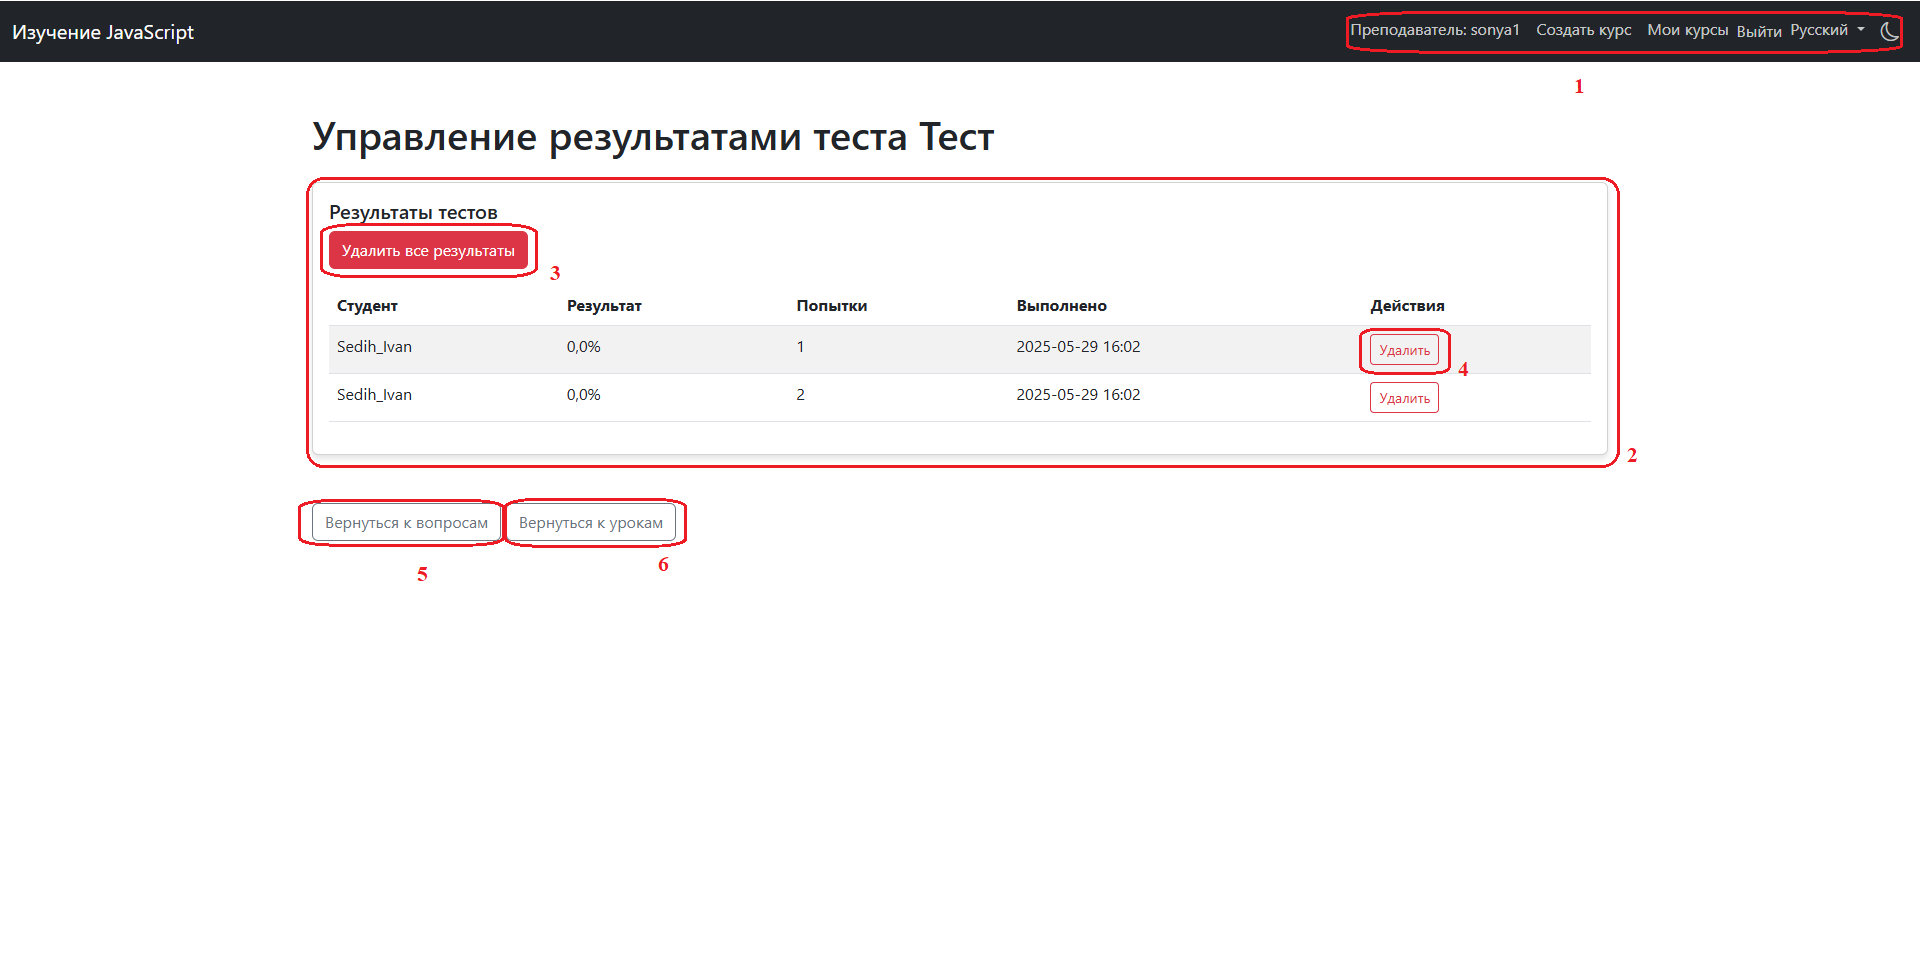
\includegraphics[width=0.7\linewidth]{images/результаты} 
	\caption{Отчёт по результатам тестов}
	\label{zotchet:image}
\end{figure}

Ключевой особенностью данного отчёта является ограничение на количество попыток прохождения теста. Если студент превышает допустимое число попыток, доступ к тесту блокируется, и система уведомляет об этом (messages.error). Каждому отчёту присваивается уникальный идентификатор, исключающий дублирование данных при формировании статистики за определённый период.

Поскольку результаты тестов фиксируются в базе данных SQLite, отчёт не подлежит обнулению или повторному формированию без вмешательства администратора. Данные о результатах автоматически передаются преподавателю через интерфейс (managetestresults), что упрощает анализ. 

Отчёт по результатам тестов необходим: 

\begin{itemize}
	\item студенту для отслеживания своего прогресса и улучшения результатов; 
	\item преподавателю для контроля успеваемости и корректировки учебного плана; 
	\item администратору системы для анализа активности пользователей и проверки корректности работы модуля тестирования.
\end{itemize}


\section{Техническое задание}
\subsection{Основание для разработки}

Основанием для разработки является задание на выпускную квалификационную работу бакалавра "<Веб-приложение для компьютерной поддержки самостоятельной работы  иностранных студентов при изучении языка программирования  JavaScript">.

\subsection{Цель и назначение разработки}

Основной задачей выпускной квалификационной работы является разработка и внедрение веб-приложения для компьютерной поддержки самостоятельной работы  иностранных студентов при изучении языка программирования  JavaScript.

Посредством внедрения веб-приложения планируется устранить существующие недостатки, связанные с неструктурированным доступом к учебным материалам, отсутствием интерактивных инструментов для практики и тестирования, а также сложностями в организации учебного процесса для иностранных студентов, включая языковые барьеры.

Цель разработки включает следующие подцели:

\begin{itemize}
\item создание единой образовательной платформы для доступа к учебным курсам, урокам и тестам;
\item обеспечение удобного и интуитивно понятного интерфейса для самостоятельного изучения JavaScript;
\item интеграция инструментов для проверки знаний, таких как тесты с автоматической оценкой;
\item оптимизация процессов управления учебным контентом для преподавателей и взаимодействия студентов с платформой.
\end{itemize}

\subsection{Функциональные задачи}

Разрабатываемая веб-платформа включает в себя следующие модули:
\begin{itemize}
\item \textbf{Курсы} — модуль для создания и управления учебными курсами, включающими уроки и тесты. Преподаватели могут добавлять, редактировать и удалять курсы, а студенты получают доступ к материалам.;
\item \textbf{Уроки} — система управления учебным контентом, позволяющая структурировать материалы курса (текст, изображения, видео) и задавать порядок уроков. Поддерживается предпросмотр уроков и их редактирование.;
\item \textbf{Тесты} — модуль для создания и прохождения интерактивных тестов. Преподаватели могут задавать вопросы и варианты ответов, а студенты проходят тесты с автоматической оценкой результатов;
\item \textbf{Результаты тестов} — инструмент для анализа успеваемости студентов. Преподаватели могут просматривать, удалять и управлять результатами тестов, включая статистику по студентам;
\item \textbf{Панель управления преподавателя} — интерфейс для управления курсами, уроками, тестами и результатами, с удобной навигацией и виджетами для быстрого доступа;
\item \textbf{Профиль пользователя} — модуль для управления учетной записью, включая настройки аватара и персональной информации;
\item \textbf{Сообщения} — система уведомлений для обратной связи (например, сообщения об успешном добавлении урока или удалении результатов);
\item \textbf{Панель управления} — страница с виджетами всех вышеперечисленных сервисов.
\end{itemize}

\subsection{Требования пользователя к интерфейсу web-сайта}

Платформа должна обеспечивать:
\begin{itemize}
    \item авторизацию;
    \item интуитивно понятную навигацию между модулями;
    \item адаптивный интерфейс для десктопных и мобильных устройств.
\end{itemize}

Композиция интерфейса пользователя представлена на рисунках ~\ref{templ:image1}, ~\ref{templ:image2}, ~\ref{templ:image3}, ~\ref{templ:image4}, ~\ref{templ:image5}, ~\ref{templ:image6}, ~\ref{templ:image7}, ~\ref{templ:image8}, ~\ref{templ:image9},  ~\ref{templ:image10}.

\begin{figure}[ht]
	\centering
	\includegraphics[width=1\linewidth]{images/курсы}
	\caption{Композиция интерфейса сервиса <<Курсы>>}
	\label{templ:image1}
\end{figure}

\begin{figure}[ht]
	\centering
	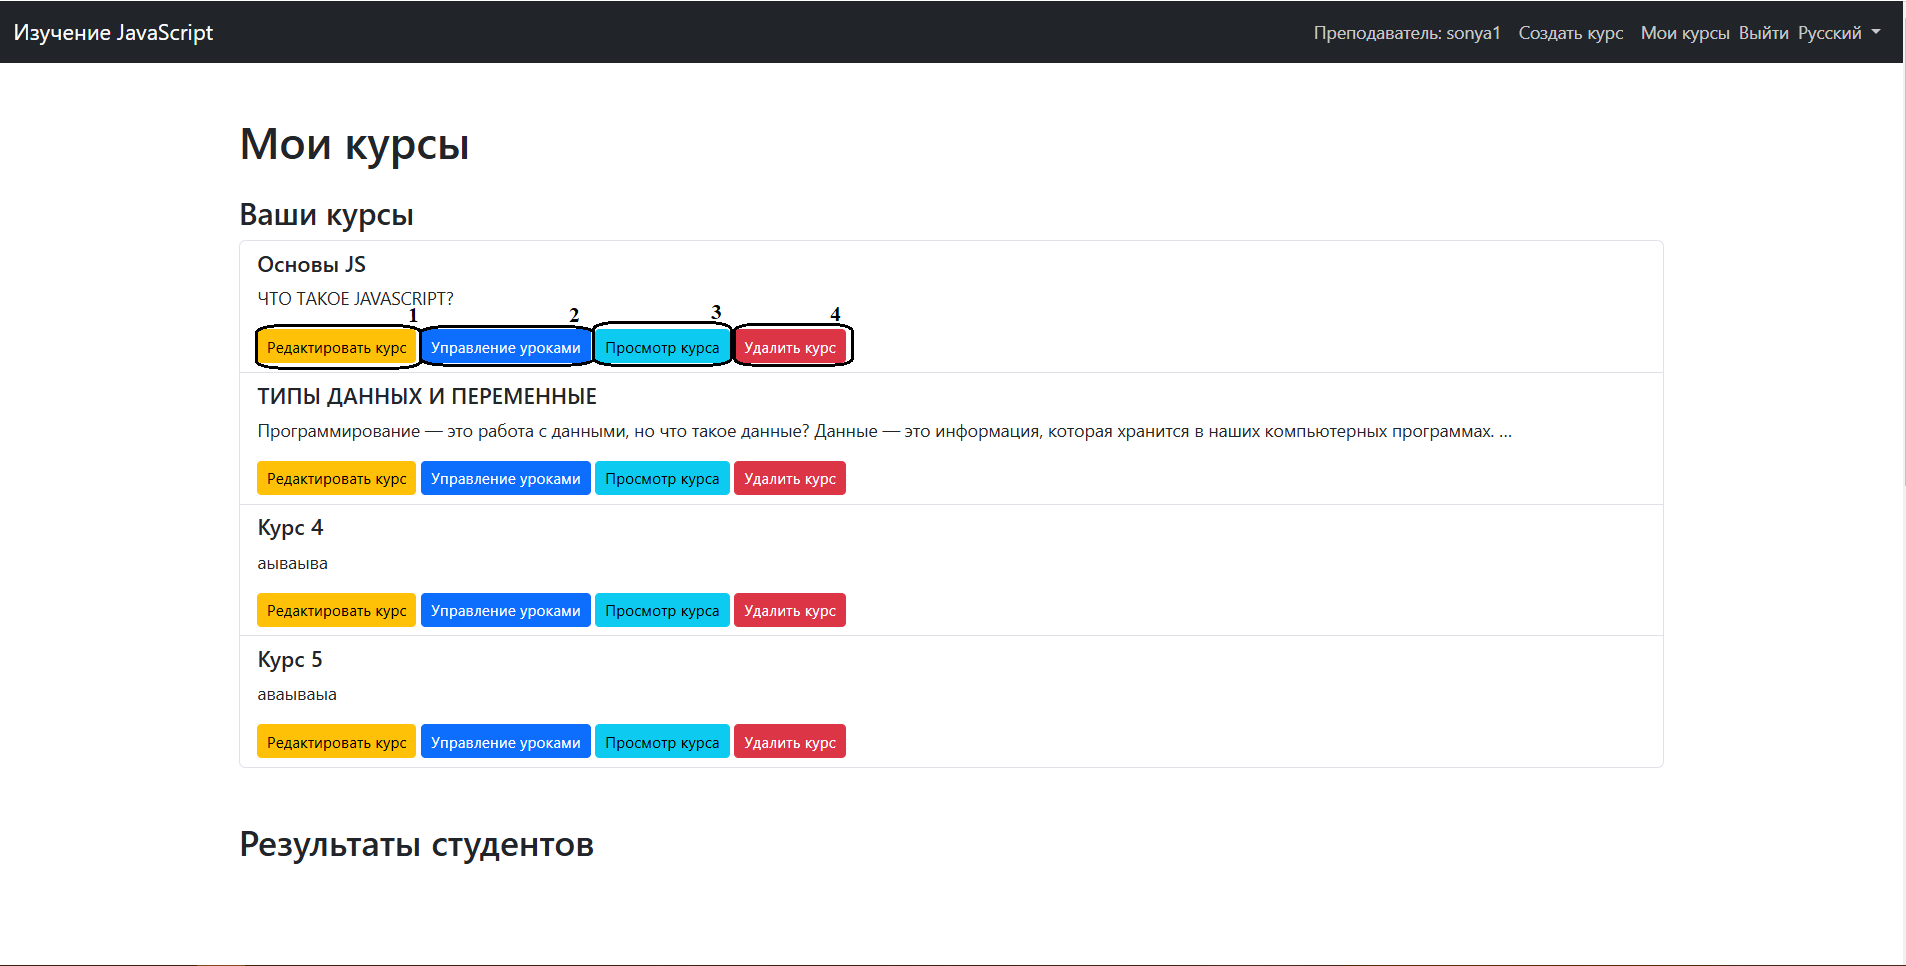
\includegraphics[width=1\linewidth]{images/учитель}
	\caption{Композиция интерфейса сервиса <<Панель управления преподавателя>>}
	\label{templ:image2}
\end{figure}

\begin{figure}[ht]
	\centering
	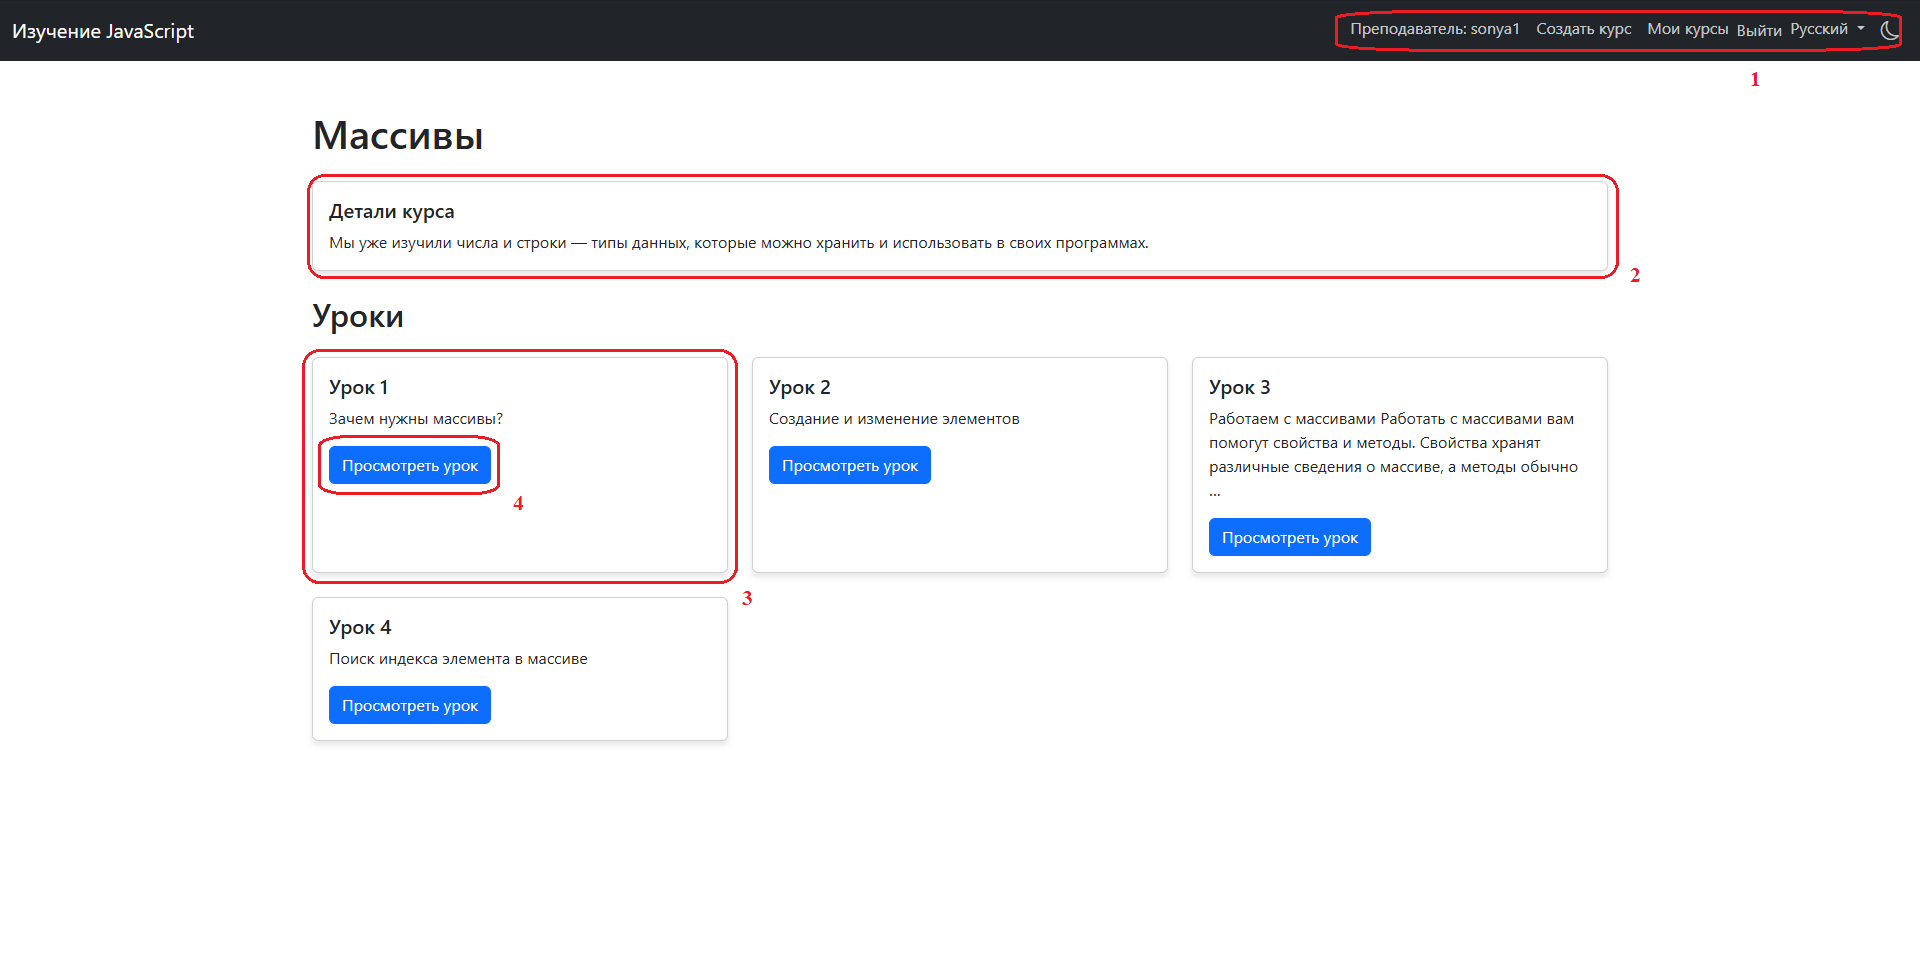
\includegraphics[width=1\linewidth]{images/уроки}
	\caption{Композиция интерфейса сервиса <<Уроки>>}
	\label{templ:image3}
\end{figure}

\begin{figure}[ht]
	\centering
	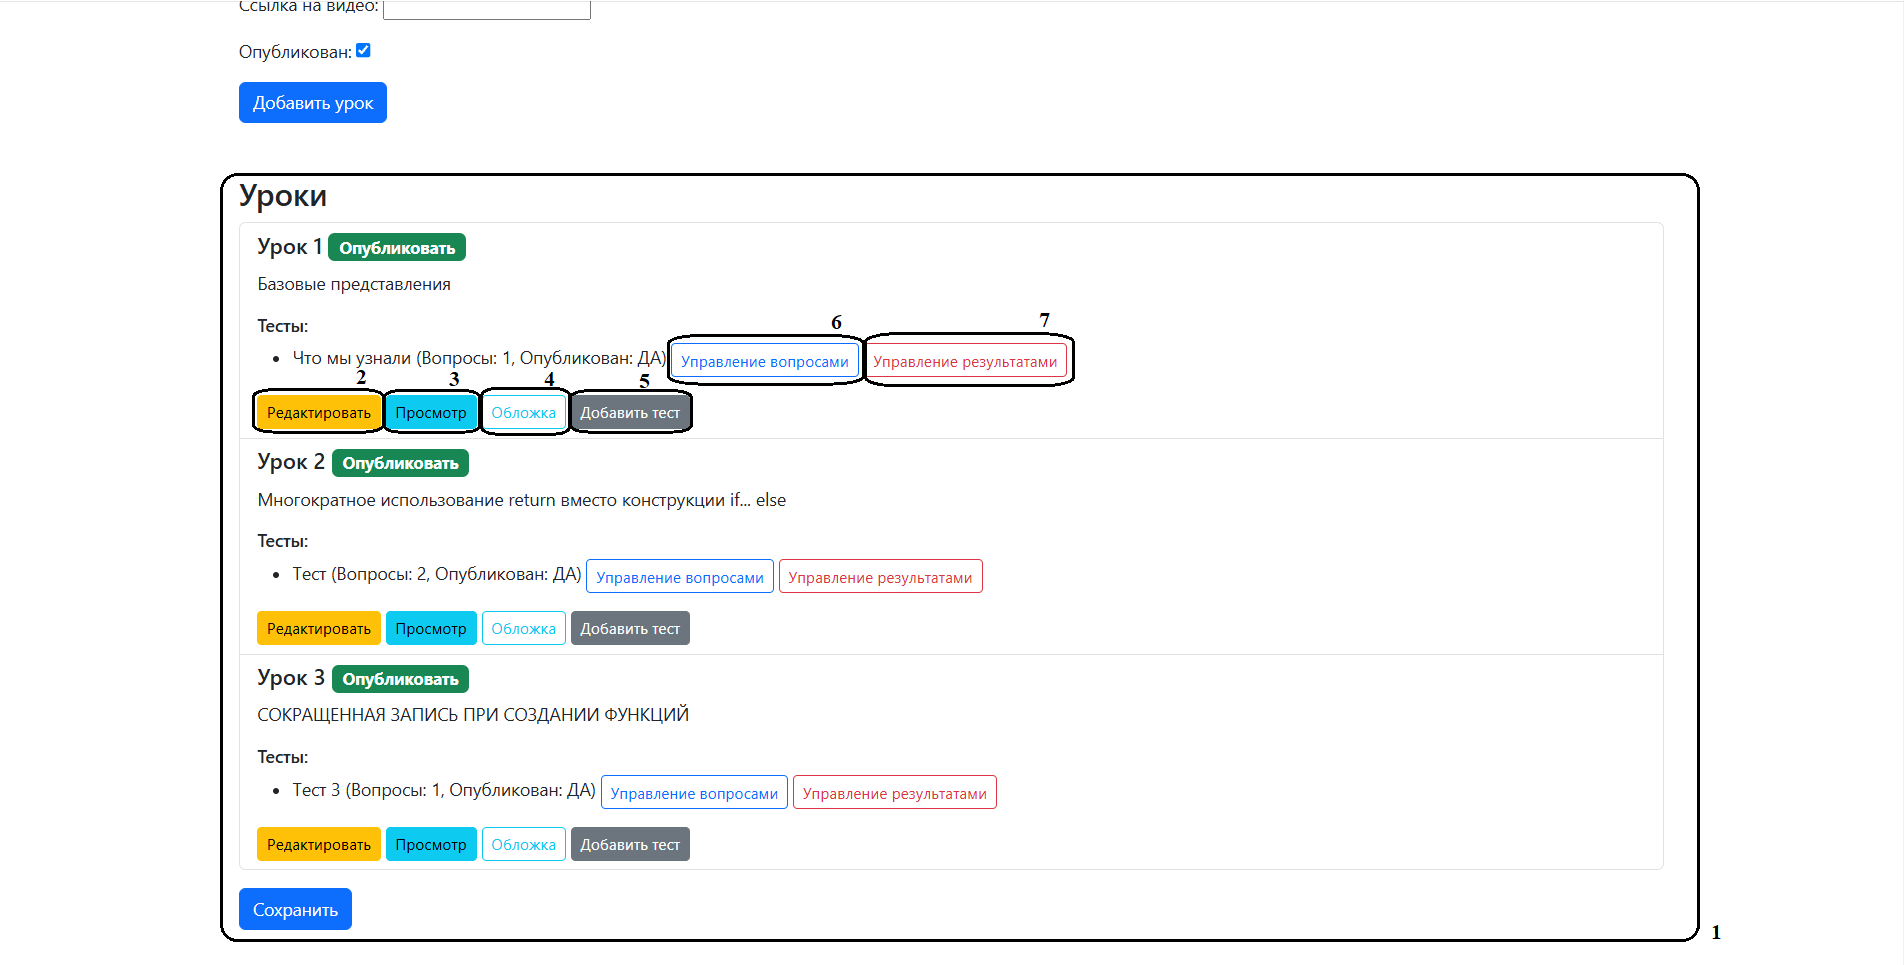
\includegraphics[width=1\linewidth]{images/Тесты}
	\caption{Композиция интерфейса сервиса <<Тесты>>}
	\label{templ:image4}
\end{figure}

\begin{figure}[ht]
	\centering
	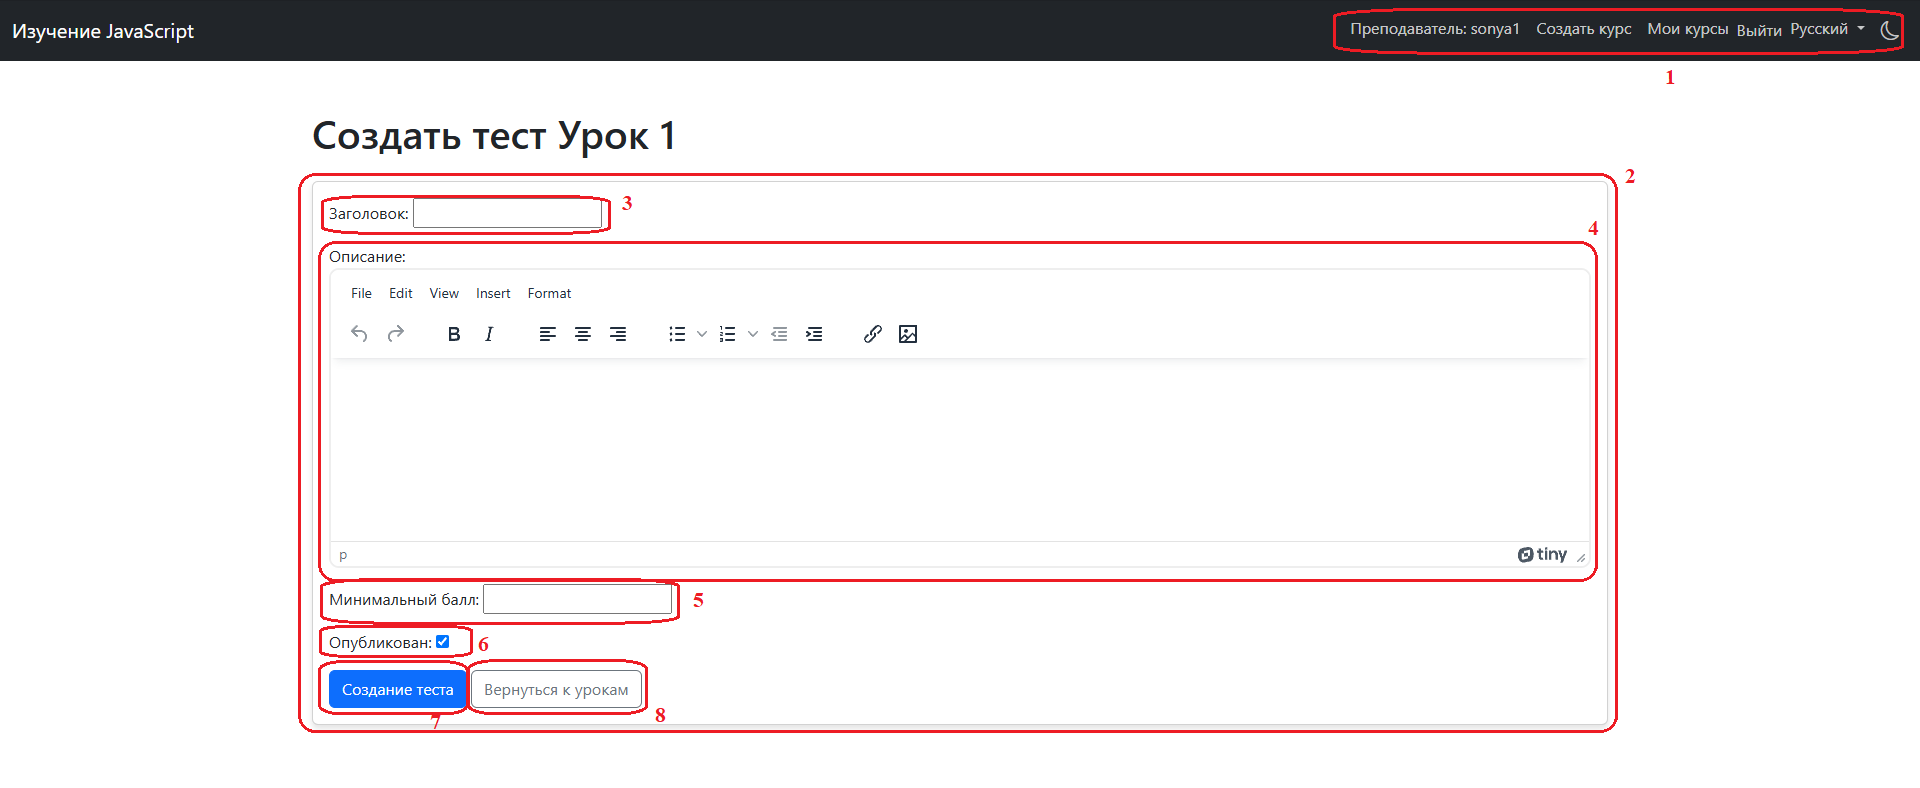
\includegraphics[width=1\linewidth]{images/создатьтест}
	\caption{Композиция интерфейса сервиса <<Создание теста>>}
	\label{templ:image5}
\end{figure}

\begin{figure}[ht]
	\centering
	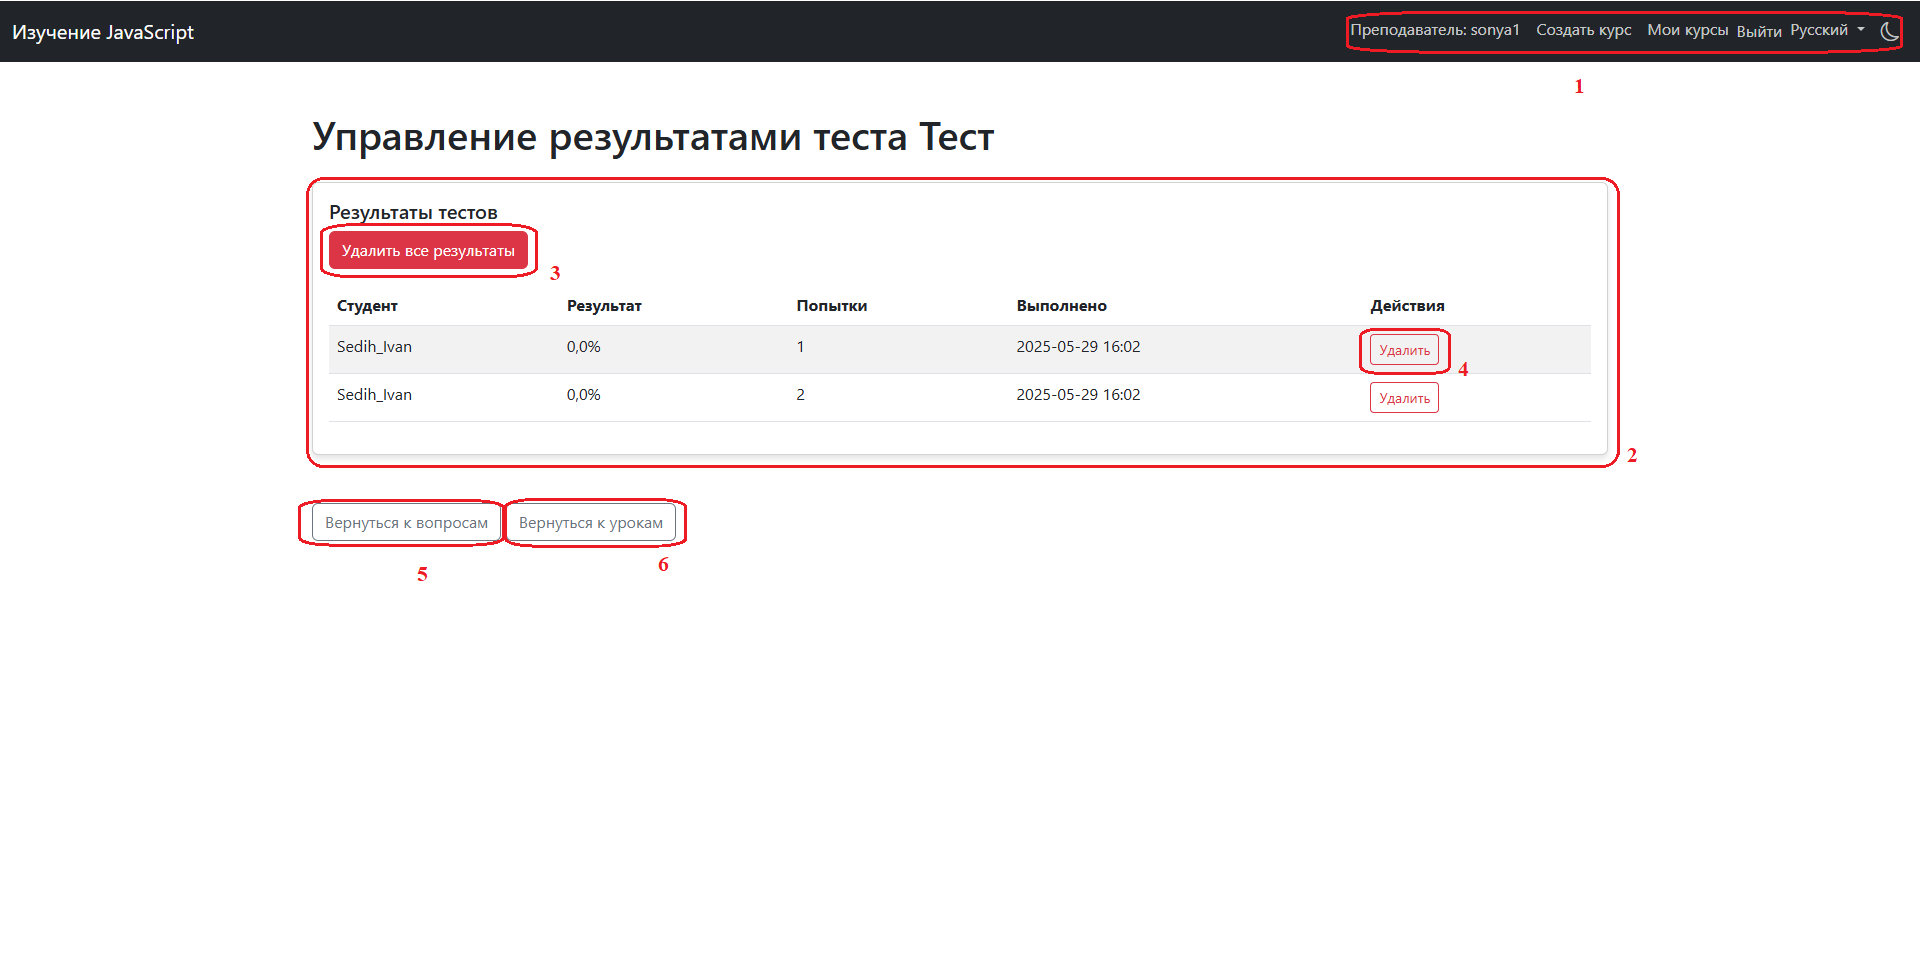
\includegraphics[width=1\linewidth]{images/результаты}
	\caption{Композиция интерфейса сервиса <<Результаты тестов>>}
	\label{templ:image6}
\end{figure}

\begin{figure}[ht]
	\centering
	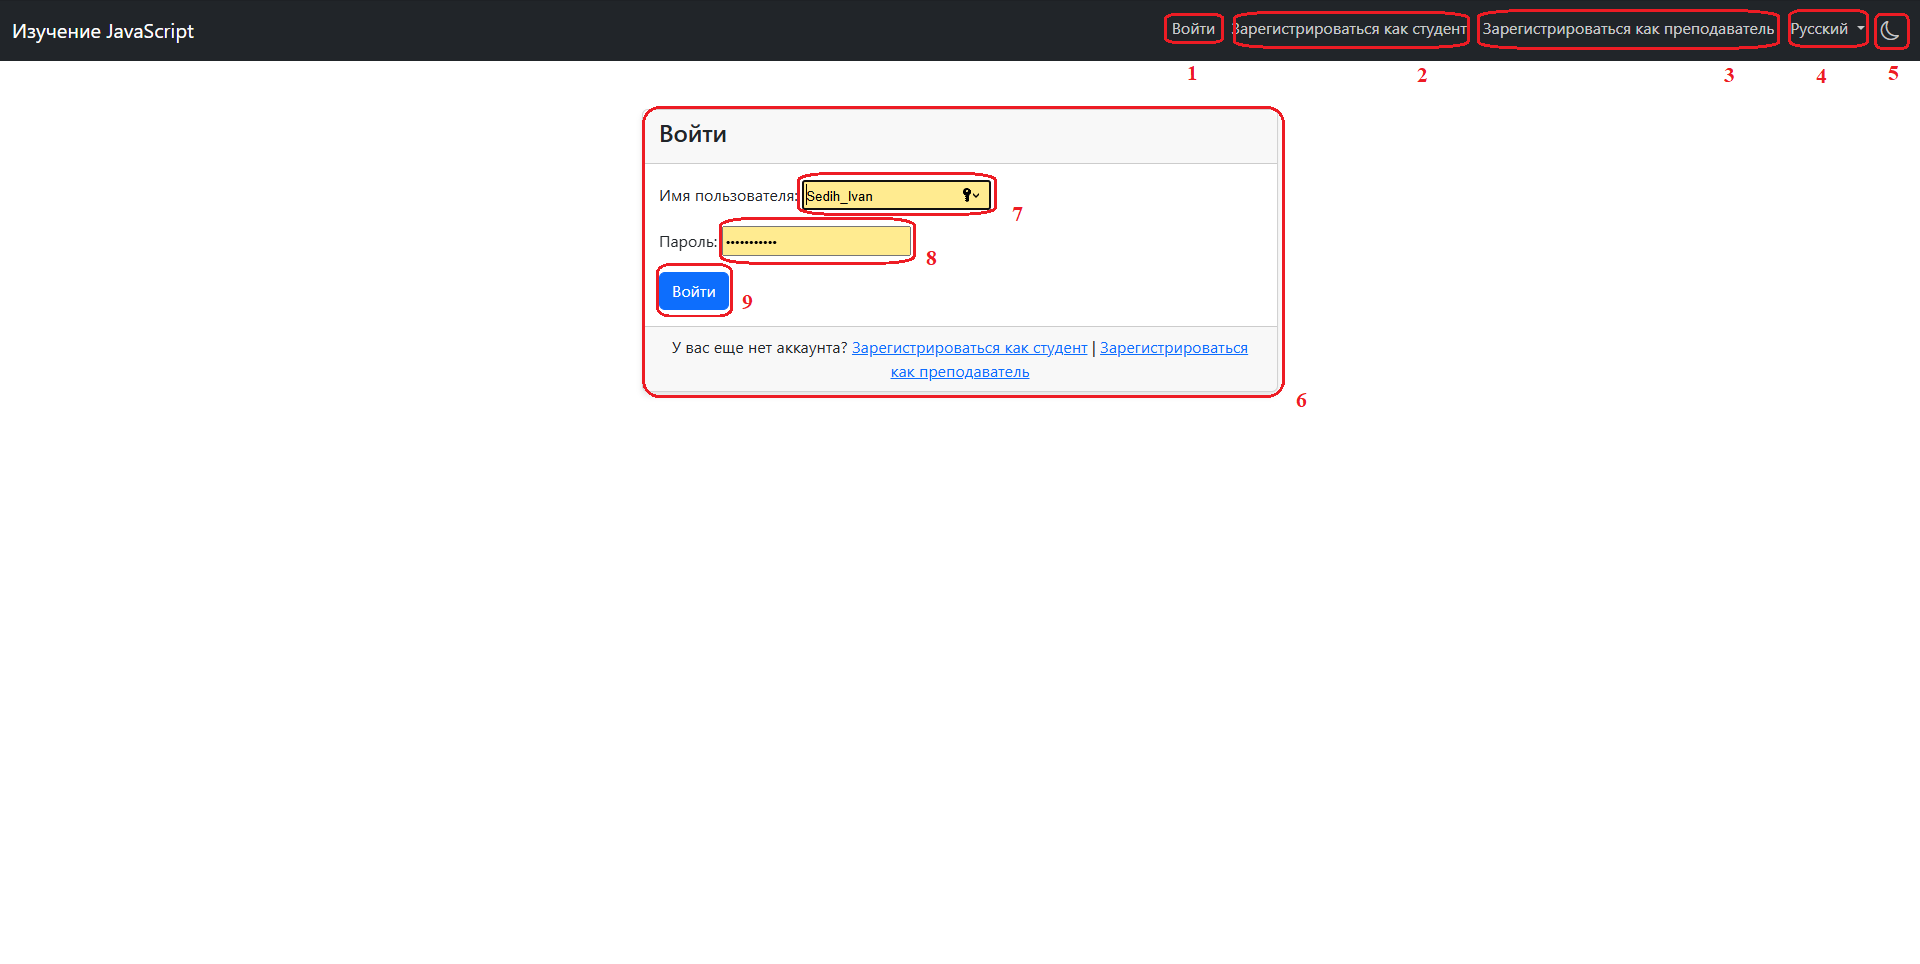
\includegraphics[width=1\linewidth]{images/Авторизация}
	\caption{Композиция интерфейса сервиса <<Авторизация>>}
	\label{templ:image7}
\end{figure}


\begin{figure}[ht]
	\centering
	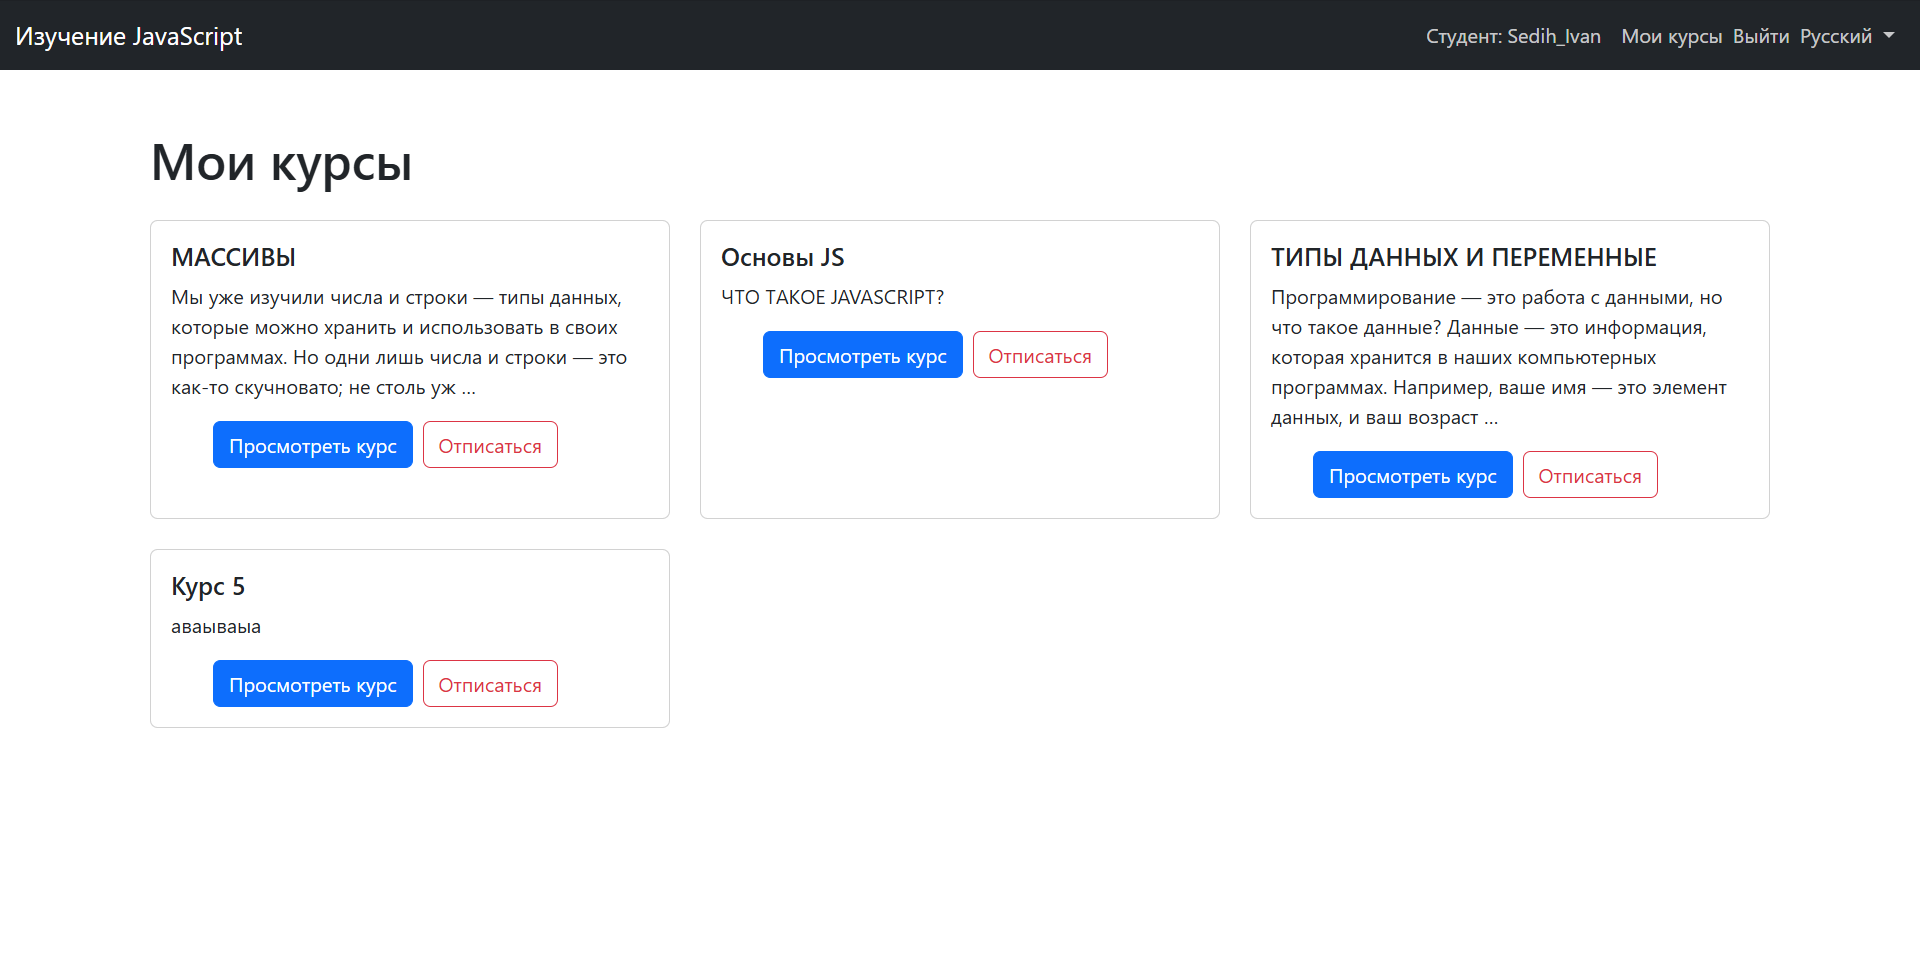
\includegraphics[width=1\linewidth]{images/профиль}
	\caption{Композиция интерфейса сервиса <<Профиль>>}
	\label{templ:image8}
\end{figure}


\begin{figure}[ht]
	\centering
	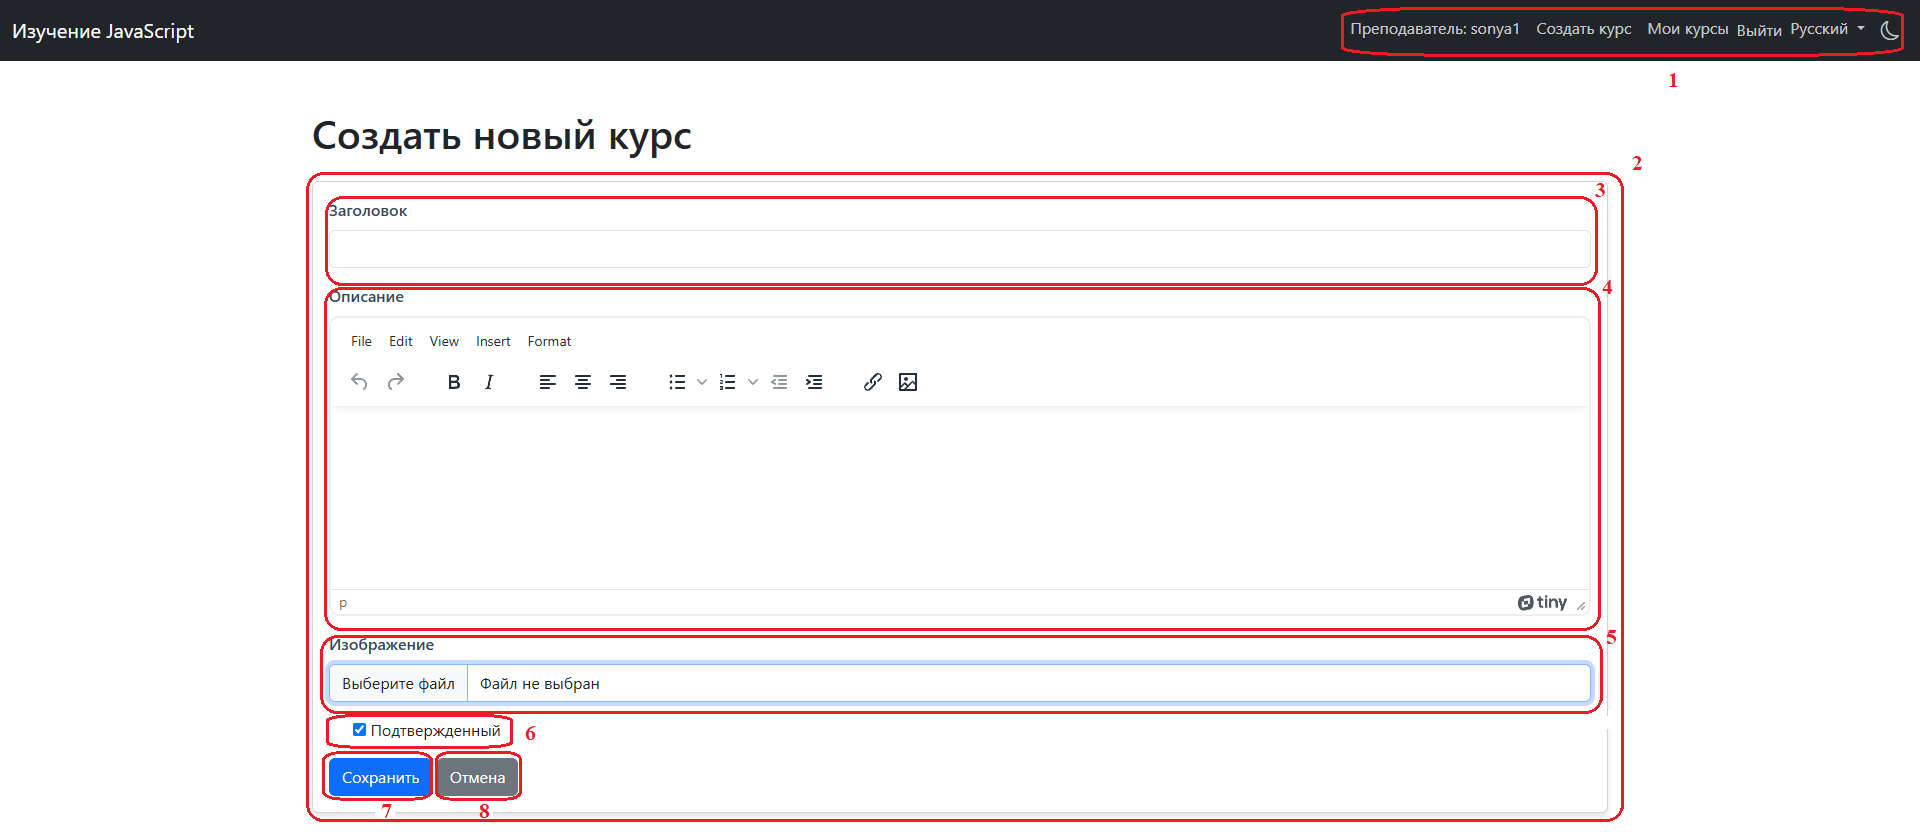
\includegraphics[width=1\linewidth]{images/создатькурс}
	\caption{Композиция интерфейса сервиса <<Создание курса>>}
	\label{templ:image9}
\end{figure}


\begin{figure}[ht]
	\centering
	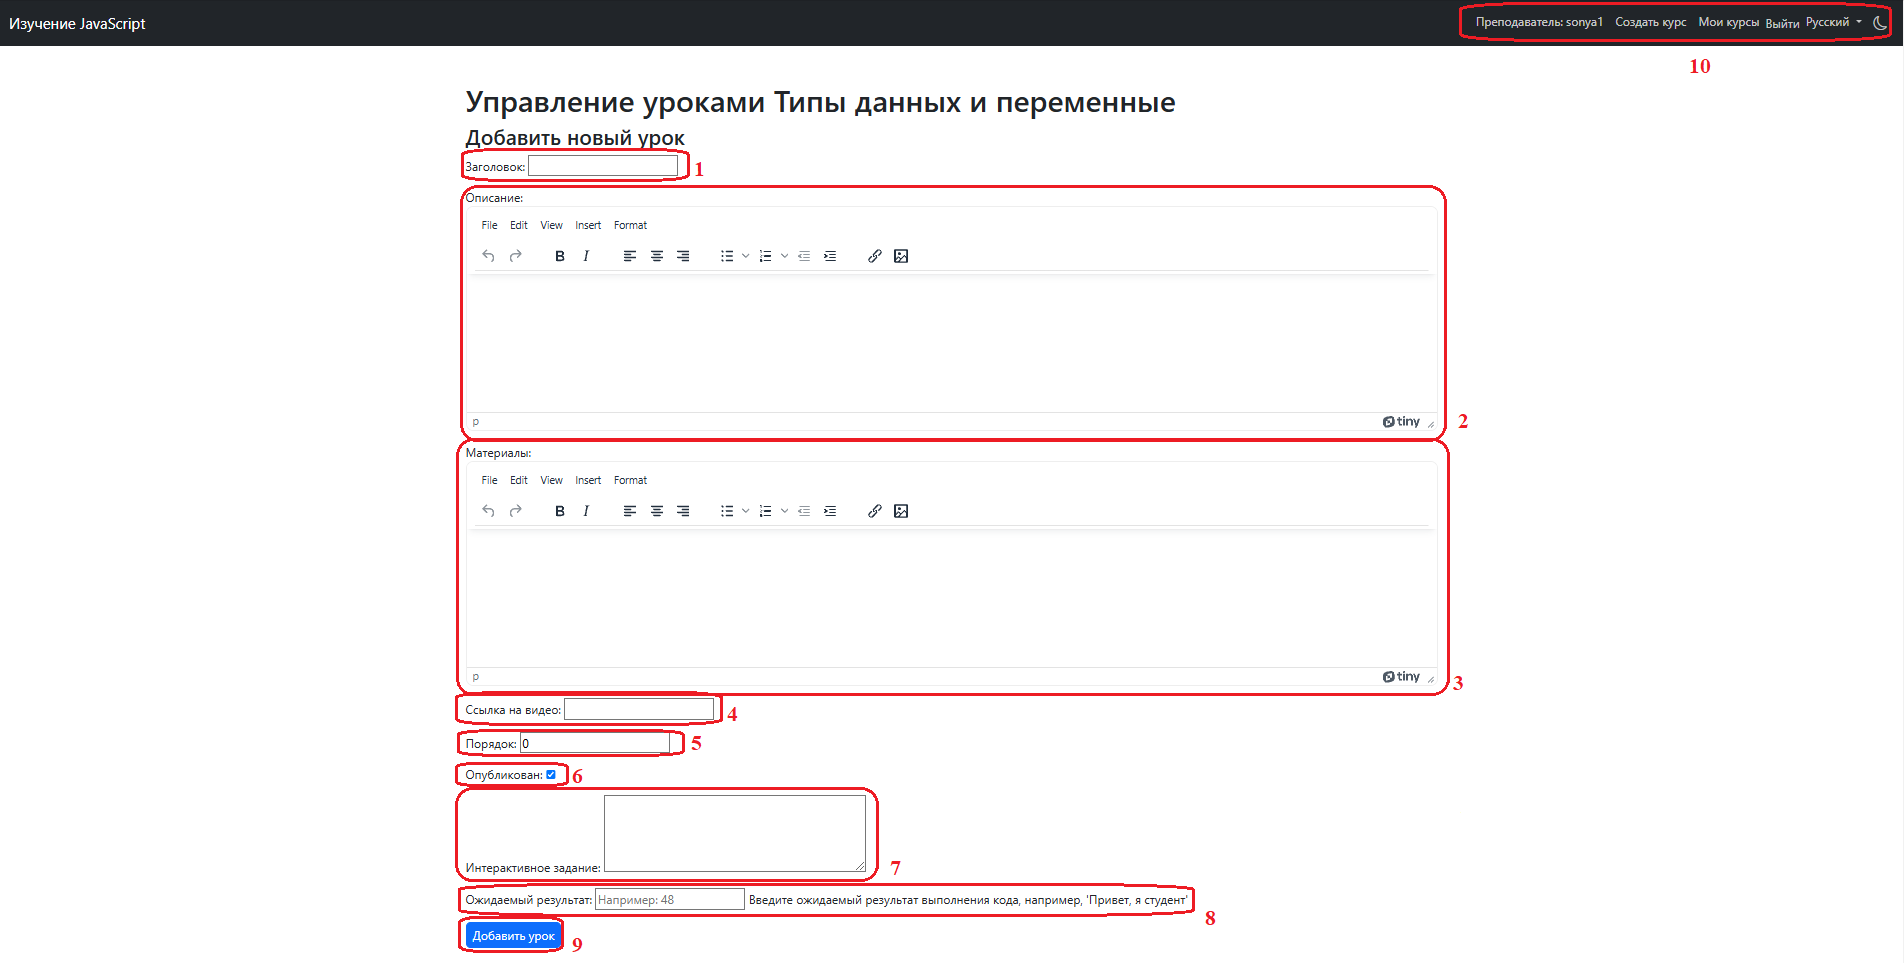
\includegraphics[width=1\linewidth]{images/создатьурок}
	\caption{Композиция интерфейса сервиса <<Создание урока>>}
	\label{templ:image10}
\end{figure}

\clearpage
\subsection{Моделирование вариантов использования}

Для разработки платформы была построена UML-диаграмма вариантов использования, отражающая взаимодействие пользователей с системой.

Основные прецеденты системы:
\begin{enumerate}
\item Авторизация и выход из системы.
\item Управление курсами.
\item Управление уроками.
\item Создание и управление тестами.
\item Прохождение тестов.
\item Просмотр результатов тестов.
\item Локализация интерфейса.

\end{enumerate}

\subsection{Требования к оформлению документации}

Разработка программной документации и программного изделия должна производиться согласно ГОСТ 19.102–77 и ГОСТ 34.601–90. Единая система программной документации.

\section{Технический проект}

\subsection{Общая характеристика организации решения задачи}

Разработанное веб-приложение представляет собой онлайн-платформу для самостоятельного изучения JavaScript иностранными студентами. Платформа реализована с использованием современных веб-технологий: HTML, CSS, JavaScript и Python (Django). Она размещается в сети Интернет (например, на домене (https://swsueducate.ru) и предоставляет единый пользовательский интерфейс для студентов и преподавателей.

Основные задачи платформы:
\begin{itemize}
	\item управление курсами и уроками;
	\item создание и проведение тестов;
	\item анализ результатов обучения;
	\item поддержка локализации для разных языков.
\end{itemize}

Система построена на клиент-серверной архитектуре:
\begin{enumerate}
	\item {Клиентская часть} (Frontend): Реализована с использованием HTML, CSS (Bootstrap для адаптивности) и JavaScript (включая Sortable.js для сортировки уроков). Отвечает за отображение интерфейса и интерактивность.
	\item {Серверная часть} (Backend): Построена на Django, обрабатывает запросы, управляет данными (через SQLite) и генерирует динамические страницы.
	\item {База данных}: SQLite хранит данные о курсах, уроках, тестах, пользователях и их прогрессе.
\end{enumerate}

\subsection{Архитектура системы}

Архитектура платформы следует модели MVC (Model-View-Controller), реализованной через Django, что обеспечивает чёткое разделение ответственности между компонентами системы.

\subsubsection{Описание архитектуры}

\begin{enumerate}
	\item {Model} (Модель): Определяет структуру данных в виде таблиц SQLite (courses\_course, courses\_lesson, courses\_test, courses\_question, courses\_answer, users\_user и др.). Модели Django обеспечивают взаимодействие с базой данных через ORM, упрощая операции создания, чтения, обновления и удаления данных (CRUD).
	\item {View} (Представление): Обрабатывает HTTP-запросы и формирует ответы. Включает функции и классы Django views, которые возвращают HTML-страницы (через шаблоны Django) или JSON-ответы для динамической загрузки данных.
	\item {Controller} (Контроллер): Реализован через маршрутизацию Django файл (urls.py), направляющую запросы к соответствующим представлениям.
\end{enumerate}

Основные компоненты системы:
\begin{enumerate}
	\item {Frontend}: Интерфейс пользователя, созданный с помощью шаблонов Django (HTML), стилей Bootstrap и JavaScript. Sortable.js используется для реализации сортировки уроков в интерфейсе преподавателя.
	\item {Backend}: Сервер Django, который управляет логикой приложения, включая аутентификацию (contrib.auth), ограничение доступа (@login\_required) и локализацию (i18n).
	\item {Database}: SQLite, содержащая реляционные таблицы для хранения данных. Использование SQLite обусловлено лёгкостью и достаточной производительностью для данного проекта.
	\item {API}: Внутренние API-методы (реализованы через Django views), обеспечивающие взаимодействие между клиентской и серверной частями, например, для загрузки списка уроков или результатов тестов.
\end{enumerate}

Архитектура представлена на диаграмме компонентов (см. рис.~\ref{diag:image}).

\begin{figure}[htp!]
	\centering{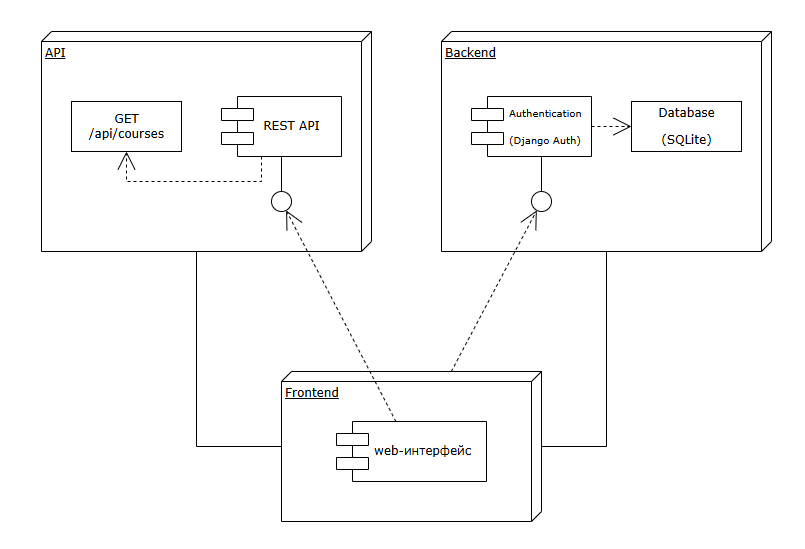
\includegraphics[width=0.7\linewidth]{images/диаграмма1}}
	\caption{Диаграмма компонентов}
	\label{diag:image}
\end{figure}

\subsection{Структура базы данных}

Проанализировав требования, выделены следующие основные сущности:
\begin{itemize}
	\item курсы;
	\item уроки;
	\item тесты;
	\item вопросы;
	\item ответы;
	\item результаты тестов;
	\item пользователи;
	\item запись на курсы;
	\item прогресс;
	\item связь пользователей и курсов.
\end{itemize}

Отношения между таблицами базы данных отражены на схеме (см. рис.~\ref{bd:image}).

\begin{landscape}
	\begin{figure}[ht]
		\centering
		\includegraphics[width=1.2\textwidth]{images/бд} 
		\caption{Структура базы данных}
		\label{bd:image}
	\end{figure}
\end{landscape}

Ниже приведены атрибуты сущностей в формате таблиц.

\begin{xltabular}{\textwidth}{|l|l|p{3.2cm}|X|}
	\caption{Атрибуты сущности <<Курсы>>\label{courses:table}}\\ \hline
	Поле & Тип & Обязательное & Описание \\ \hline
	\endfirsthead
	\continuecaption{Продолжение таблицы \ref{courses:table}}\\ \hline
	Поле & Тип & Обязательное & Описание \\ \hline
	\endhead
	id & Integer & true & Уникальный идентификатор курса \\ \hline
	title & String & true & Название курса \\ \hline
	description & Text & true & Описание курса \\ \hline
	image & String & false & Путь к изображению курса \\ \hline
	isactive & Boolean & true & Признак активности курса \\ \hline
	createdat & DateTime & true & Дата создания курса \\ \hline
	teacherid & ForeignKey & true & Преподаватель (ссылка на таблицу Пользователи) \\ \hline
\end{xltabular}

\begin{xltabular}{\textwidth}{|l|l|p{3.2cm}|X|}
	\caption{Атрибуты сущности <<Уроки>>\label{lessons:table}}\\ \hline
	Поле & Тип & Обязательное & Описание \\ \hline
	\endfirsthead
	\continuecaption{Продолжение таблицы \ref{lessons:table}}\\ \hline
	Поле & Тип & Обязательное & Описание \\ \hline
	\endhead
	id & Integer & true & Уникальный идентификатор урока \\ \hline
	courseid & ForeignKey & true & Курс, к которому относится урок (ссылка на таблицу Курсы) \\ \hline
	title & String & true & Название урока \\ \hline
	description & Text & false & Описание урока \\ \hline
	content & Text & true & Содержимое урока (текст, HTML) \\ \hline
	videourl & String & true & Ссылка на видео урока \\ \hline
	order & Integer & true & Порядок урока в курсе \\ \hline
	ispublished & Boolean & true & Признак публикации урока \\ \hline
	createdat & DateTime & true & Дата создания урока \\ \hline
\end{xltabular}


\begin{xltabular}{\textwidth}{|l|l|p{3.2cm}|X|}
	\caption{Атрибуты сущности <<Тесты>>\label{tests:table}}\\ \hline
	Поле & Тип & Обязательное & Описание \\ \hline
	\endfirsthead
	\continuecaption{Продолжение таблицы \ref{tests:table}}\\ \hline
	Поле & Тип & Обязательное & Описание \\ \hline
	\endhead
	id & Integer & true & Уникальный идентификатор теста \\ \hline
	lessonid & ForeignKey & true & Урок, к которому относится тест (ссылка на таблицу Уроки) \\ \hline
	title & String & true & Название теста \\ \hline
	description & Text & true & Описание теста \\ \hline
	questions & Array & false & Список вопросов (JSON или связанные модели) \\ \hline
	isactive & Boolean & true & Признак активности теста \\ \hline
	passingscore & Integer & true & Проходной балл (в процентах) \\ \hline
	createdat & DateTime & false & Дата создания теста (может отсутствовать) \\ \hline
\end{xltabular}

\begin{xltabular}{\textwidth}{|l|l|p{3.2cm}|X|}
	\caption{Атрибуты сущности <<Результаты тестов>>\label{test_results:table}}\\ \hline
	Поле & Тип & Обязательное & Описание \\ \hline
	\endfirsthead
	\continuecaption{Продолжение таблицы \ref{test_results:table}}\\ \hline
	Поле & Тип & Обязательное & Описание \\ \hline
	\endhead
	id & Integer & true & Уникальный идентификатор результата \\ \hline
	studentid & ForeignKey & true & Студент (ссылка на таблицу Пользователи) \\ \hline
	lessonid & ForeignKey & true & Урок, связанный с тестом (ссылка на таблицу Уроки) \\ \hline
	score & Float & true & Оценка (в процентах или дробное значение) \\ \hline
	attempts & Integer & true & Количество попыток \\ \hline
	answers & Text & true & Ответы (в формате JSON) \\ \hline
	completedat & DateTime & true & Дата завершения теста \\ \hline
\end{xltabular}

\begin{xltabular}{\textwidth}{|l|l|p{3.2cm}|X|}
	\caption{Атрибуты сущности <<Пользователи>>\label{users:table}}\\ \hline
	Поле & Тип & Обязательное & Описание \\ \hline
	\endfirsthead
	\continuecaption{Продолжение таблицы \ref{users:table}}\\ \hline
	Поле & Тип & Обязательное & Описание \\ \hline
	\endhead
	id & Integer & true & Уникальный идентификатор пользователя \\ \hline
	username & String & true & Имя пользователя \\ \hline
	email & String & true & Электронная почта \\ \hline
	isteacher & Boolean & true & Признак преподавателя \\ \hline
	password & String & true & Хэшированный пароль пользователя \\ \hline
	lastlogin & DateTime & false & Дата последнего входа \\ \hline
	issuperuser & Boolean & true & Признак суперпользователя \\ \hline
	firstname & String & true & Имя пользователя \\ \hline
	lastname & String & true & Фамилия пользователя \\ \hline
	isstaff & Boolean & true & Признак персонала \\ \hline
	isactive & Boolean & true & Признак активности пользователя \\ \hline
	datejoined & DateTime & true & Дата регистрации \\ \hline
	isstudent & Boolean & true & Признак студента \\ \hline
	isadmin & Boolean & true & Признак администратора \\ \hline
\end{xltabular}

\begin{xltabular}{\textwidth}{|l|l|p{3.2cm}|X|}
	\caption{Атрибуты сущности <<Запись на курсы>>\label{enrollments:table}}\\ \hline
	Поле & Тип & Обязательное & Описание \\ \hline
	\endfirsthead
	\continuecaption{Продолжение таблицы \ref{enrollments:table}}\\ \hline
	Поле & Тип & Обязательное & Описание \\ \hline
	\endhead
	id & Integer & true & Уникальный идентификатор записи \\ \hline
	enrolledat & DateTime & true & Дата записи на курс \\ \hline
	courseid & ForeignKey & true & Курс (ссылка на таблицу Курсы) \\ \hline
	studentid & ForeignKey & true & Студент (ссылка на таблицу Пользователи) \\ \hline
\end{xltabular}

\begin{xltabular}{\textwidth}{|l|l|p{3.2cm}|X|}
	\caption{Атрибуты сущности <<Прогресс>>\label{progress:table}}\\ \hline
	Поле & Тип & Обязательное & Описание \\ \hline
	\endfirsthead
	\continuecaption{Продолжение таблицы \ref{progress:table}}\\ \hline
	Поле & Тип & Обязательное & Описание \\ \hline
	\endhead
	id & Integer & true & Уникальный идентификатор прогресса \\ \hline
	completed & Boolean & true & Признак завершения урока \\ \hline
	completedat & DateTime & false & Дата завершения урока \\ \hline
	lessonid & ForeignKey & true & Урок (ссылка на таблицу Уроки) \\ \hline
	studentid & ForeignKey & true & Студент (ссылка на таблицу Пользователи) \\ \hline
\end{xltabular}

\begin{xltabular}{\textwidth}{|l|l|p{3.2cm}|X|}
	\caption{Атрибуты сущности <<Вопросы>>\label{questions:table}}\\ \hline
	Поле & Тип & Обязательное & Описание \\ \hline
	\endfirsthead
	\continuecaption{Продолжение таблицы \ref{questions:table}}\\ \hline
	Поле & Тип & Обязательное & Описание \\ \hline
	\endhead
	id & Integer & true & Уникальный идентификатор вопроса \\ \hline
	testid & ForeignKey & true & Тест (ссылка на таблицу Тесты) \\ \hline
	text & Text & true & Текст вопроса \\ \hline
	questiontype & String & true & Тип вопроса (например, выбор, текст) \\ \hline
	points & Integer & true & Баллы за вопрос \\ \hline
\end{xltabular}

\begin{xltabular}{\textwidth}{|l|l|p{3.2cm}|X|}
	\caption{Атрибуты сущности <<Ответы>>\label{answers:table}}\\ \hline
	Поле & Тип & Обязательное & Описание \\ \hline
	\endfirsthead
	\continuecaption{Продолжение таблицы \ref{answers:table}}\\ \hline
	Поле & Тип & Обязательное & Описание \\ \hline
	\endhead
	id & Integer & true & Уникальный идентификатор ответа \\ \hline
	questionid & ForeignKey & true & Вопрос (ссылка на таблицу Вопросы) \\ \hline
	text & Text & true & Текст ответа \\ \hline
	iscorrect & Boolean & true & Признак правильности ответа \\ \hline
	order & Integer & true & Порядок ответа \\ \hline
\end{xltabular}

\begin{xltabular}{\textwidth}{|l|l|p{3.2cm}|X|}
	\caption{Атрибуты сущности <<Связь пользователей и курсов>>\label{user_courses:table}}\\ \hline
	Поле & Тип & Обязательное & Описание \\ \hline
	\endfirsthead
	\continuecaption{Продолжение таблицы \ref{user_courses:table}}\\ \hline
	Поле & Тип & Обязательное & Описание \\ \hline
	\endhead
	id & Integer & true & Уникальный идентификатор записи \\ \hline
	userid & ForeignKey & true & Пользователь (ссылка на таблицу Пользователи) \\ \hline
	courseid & ForeignKey & true & Курс (ссылка на таблицу Курсы) \\ \hline
\end{xltabular}

Экземпляры этих сущностей реализуются в информационных блоках пользовательского интерфейса. Атрибуты сущностей отображаются в полях, свойствах и компонентах соответствующих элементов.

\subsection{Обоснование выбора технологий}

Для реализации платформы выбраны следующие технологии:
\begin{enumerate}
	\item {Python и Django}: Python обеспечивает простоту и читаемость кода, а Django предоставляет мощный ORM, встроенную аутентификацию (contrib.auth) и локализацию (i18n). Это ускоряет разработку серверной части и упрощает управление данными.
	\item {JavaScript и Sortable.js}: JavaScript отвечает за клиентскую интерактивность (динамическое обновление страниц, обработка событий), а Sortable.js позволяет реализовать сортировку уроков.
	\item {HTML и Bootstrap}: HTML формирует структуру страниц, а Bootstrap обеспечивает адаптивный дизайн, совместимый с различными устройствами.
	\item {SQLite}: Лёгкая реляционная база данных, подходящая для небольшого проекта. SQLite поддерживает все необходимые операции через Django ORM.
\end{enumerate}

Эти технологии выбраны благодаря их совместимости, простоте интеграции и соответствию требованиям проекта. Python и Django обеспечивают надёжную серверную часть, JavaScript и Bootstrap — удобный и отзывчивый интерфейс, а SQLite — эффективное хранение данных.




\ifПрактика{}\else{
   \section{Рабочий проект}


\subsection{Спецификация компонентов и классов системы}

\subsubsection{Спецификация класса User}
User (Компонент управления пользователями) \\
Описание: Представляет пользователя системы (студента или преподавателя). Используется для аутентификации, управления ролями и отслеживания активности пользователей. Расширяет встроенную модель Django AbstractUser.

Валидация данных: 
\begin{itemize}
	\item поля username, email, password валидируются через встроенные механизмы Django (django.contrib.auth); 
	\item поля isstudent и isteacher — булевы, только одно из них может быть True (проверяется на уровне форм, например, StudentSignUpForm); 
\end{itemize}

Безопасность: 
\begin{itemize}
	\item доступ к данным пользователя ограничен через декораторы (loginrequired, teacherrequired, studentrequired) в представлениях; 
\end{itemize}

Уведомления: 
\begin{itemize}
	\item уведомления о действиях пользователя (например, регистрация, смена пароля) отображаются через Django messages framework в представлениях; 
\end{itemize}

Основные методы: 
\begin{itemize}
	\item str(): возвращает имя пользователя (username); 
	\item hasperm(perm, obj=None): проверяет права доступа пользователя; 
	\item save(): переопределяется для автоматической проверки ролей (isstudent, isteacher) перед сохранением; 
\end{itemize}

Зависимости: 
\begin{itemize}
	\item встроенная модель Django (django.contrib.auth.models.AbstractUser); 
	\item связан с моделями Enrollment, StudentProgress, UserAchievement через внешние ключи; 
	\item используется в формах (StudentSignUpForm, TeacherSignUpForm) и представлениях (StudentSignUpView, TeacherSignUpView); 
\end{itemize}

Таблица 4.1 – Данные класса User \\
\begin{tabular}{|p{4cm}|p{8cm}|}
	\hline
	Данные & Описание \\
	\hline
	username & уникальное имя пользователя; \\
	email & электронная почта пользователя; \\
	password & хэшированный пароль пользователя; \\
	isstudent & булево поле, указывающее, является ли пользователь студентом; \\
	isteacher & булево поле, указывающее, является ли пользователь преподавателем; \\
	fields & поля модели User, доступные для заполнения (username, email, password, isstudent, isteacher); \\
	\hline
\end{tabular}

Таблица 4.2 – Методы класса User \\
\begin{tabular}{|p{4cm}|p{8cm}|}
	\hline
	Метод & Описание \\
	\hline
	str() & возвращает имя пользователя (username); \\
	hasperm(perm, obj=None) & проверяет права доступа пользователя на основе роли и разрешений; \\
	save() & переопределяет сохранение для проверки ролей (isstudent, isteacher); \\
	\hline
\end{tabular}

\subsubsection{Спецификация класса Course}
Course (Компонент управления курсами) \\
Описание: Представляет учебный курс, созданный преподавателем. Хранит информацию о названии, описании, изображении и статусе публикации. Используется для организации уроков и тестов.

Валидация данных: 
\begin{itemize}
	\item поля title, description валидируются через Django-формы (CourseForm); 
	\item поле image проверяется на корректный формат (например, JPEG, PNG) через FileField валидаторы; 
\end{itemize}

Связи: 
\begin{itemize}
	\item связан с моделью User через поле creator (внешний ключ); 
	\item связан с моделями Lesson и Enrollment через внешние ключи (course); 
\end{itemize}

Безопасность: 
\begin{itemize}
	\item доступ к редактированию курса ограничен через проверку creator в представлениях (например, CourseUpdateView); 
	\item студенты могут просматривать только опубликованные курсы (isactive=True); 
\end{itemize}

Уведомления: 
\begin{itemize}
	\item уведомления о создании или обновлении курса отображаются через Django messages framework в представлениях (например, "Курс успешно обновлён"); 
\end{itemize}

Основные методы: 
\begin{itemize}
	\item str(): возвращает название курса (title); 
	\item getabsoluteurl(): возвращает URL курса для маршрутизации (например, /courses/<id>/); 
	\item save(): переопределяет сохранение для обработки изображения; 
\end{itemize}

Зависимости: 
\begin{itemize}
	\item взаимодействует с моделями Lesson, Test и Enrollment; 
	\item используется в шаблонах (coursedetail.html, courseform.html) с CKEditor для редактирования описания; 
	\item зависит от defaultstorage для хранения изображений; 
\end{itemize}

Таблица 4.3 – Данные класса Course \\
\begin{tabular}{|p{4cm}|p{8cm}|}
	\hline
	Данные & Описание \\
	\hline
	title & название курса; \\
	description & описание курса (форматируется через CKEditor); \\
	image & изображение курса (FileField); \\
	isactive & булево поле, указывающее статус публикации курса; \\
	creator & внешний ключ на User (преподаватель, создавший курс); \\
	fields & поля модели Course, доступные для заполнения (title, description, image, isactive, creator); \\
	\hline
\end{tabular}

Таблица 4.4 – Методы класса Course \\
\begin{tabular}{|p{4cm}|p{8cm}|}
	\hline
	Метод & Описание \\
	\hline
	str() & возвращает название курса (title); \\
	getabsoluteurl() & возвращает URL курса для маршрутизации; \\
	save() & переопределяет сохранение для обработки изображения; \\
	\hline
\end{tabular}

\subsubsection{Спецификация класса Lesson}
Lesson (Компонент управления уроками) \\
Описание: Представляет урок в рамках курса. Хранит информацию о заголовке, описании, содержимом, видео, упражнении и порядке отображения. Используется для структурирования учебного материала.

Валидация данных: 
\begin{itemize}
	\item поля title, description, content валидируются через Django-формы (LessonForm); 
	\item поле videourl проверяется на корректность через валидаторы Django; 
\end{itemize}

Связи: 
\begin{itemize}
	\item связан с моделью Course через поле course (внешний ключ); 
	\item связан с моделями Test и StudentProgress через внешние ключи (lesson); 
\end{itemize}

Безопасность: 
\begin{itemize}
	\item доступ к редактированию урока ограничен через проверку creator курса в представлениях (например, LessonUpdateView); 
	\item студенты имеют доступ только к опубликованным урокам (ispublished=True); 
\end{itemize}

Уведомления: 
\begin{itemize}
	\item уведомления о создании или обновлении урока отображаются через Django messages framework (например, "Урок успешно добавлен"); 
\end{itemize}

Основные методы: 
\begin{itemize}
	\item str(): возвращает название урока (title); 
	\item save(): переопределяет сохранение для проверки порядка (order); 
\end{itemize}

Зависимости: 
\begin{itemize}
	\item взаимодействует с моделями Course, Test и StudentProgress; 
	\item используется в шаблонах (lessondetail.html) с CKEditor для редактирования контента; 
\end{itemize}

Таблица 4.5 – Данные класса Lesson \\
\begin{tabular}{|p{4cm}|p{8cm}|}
	\hline
	Данные & Описание \\
	\hline
	title & название урока; \\
	description & описание урока; \\
	content & содержимое урока (форматируется через CKEditor); \\
	videourl & ссылка на видео урока; \\
	order & порядок урока в курсе; \\
	ispublished & булево поле, указывающее статус публикации урока; \\
	exercise & интерактивное упражнение урока; \\
	expectedresult & ожидаемый результат упражнения; \\
	course & внешний ключ на Course; \\
	fields & поля модели Lesson, доступные для заполнения (title, description, content, videourl, order, ispublished, exercise, expectedresult, course); \\
	\hline
\end{tabular}

Таблица 4.6 – Методы класса Lesson \\
\begin{tabular}{|p{4cm}|p{8cm}|}
	\hline
	Метод & Описание \\
	\hline
	str() & возвращает название урока (title); \\
	save() & переопределяет сохранение для проверки порядка (order); \\
	\hline
\end{tabular}

\subsubsection{Спецификация класса Test}
Test (Компонент управления тестами) \\
Описание: Представляет тест, связанный с уроком. Хранит информацию о названии, описании, проходном балле и статусе активности. Используется для проверки знаний студентов.

Валидация данных: 
\begin{itemize}
	\item поля title, description валидируются через Django-формы (TestForm); 
	\item поле passingscore проверяется на положительное значение через валидаторы;
\end{itemize}

Связи: 
\begin{itemize}
	\item связан с моделью Lesson через поле lesson (внешний ключ); 
	\item связан с моделями Question и TestResult через внешние ключи (test); 
\end{itemize}

Безопасность: 
\begin{itemize}
	\item доступ к редактированию теста ограничен через проверку creator урока в представлениях (например, createtest); 
	\item студенты могут проходить только активные тесты (isactive=True); 
\end{itemize}

Уведомления: 
\begin{itemize}
	\item уведомления о создании теста отображаются через Django messages framework (например, "Тест успешно создан"); 
\end{itemize}

Основные методы: 
\begin{itemize}
	\item str(): возвращает название теста (title); 
	\item save(): переопределяет сохранение для проверки passingscore; 
\end{itemize}

Зависимости: 
\begin{itemize}
	\item взаимодействует с моделями Lesson, Question и TestResult; 
	\item используется в шаблонах (testform.html) и представлениях (createtest); 
\end{itemize}

Таблица 4.7 – Данные класса Test \\
\begin{tabular}{|p{4cm}|p{8cm}|}
	\hline
	Данные & Описание \\
	\hline
	title & название теста; \\
	description & описание теста; \\
	passingscore & проходной балл теста; \\
	isactive & булево поле, указывающее статус активности теста; \\
	lesson & внешний ключ на Lesson; \\
	fields & поля модели Test, доступные для заполнения (title, description, passingscore, isactive, lesson); \\
	\hline
\end{tabular}

Таблица 4.8 – Методы класса Test \\
\begin{tabular}{|p{4cm}|p{8cm}|}
	\hline
	Метод & Описание \\
	\hline
	str() & возвращает название теста (title); \\
	save() & переопределяет сохранение для проверки passingscore; \\
	\hline
\end{tabular}

\subsubsection{Спецификация класса Question}
Question (Компонент управления вопросами теста) \\
Описание: Представляет вопрос в тесте. Хранит текст вопроса, тип вопроса (одиночный, множественный, текстовый) и баллы за правильный ответ.

Валидация данных: 
\begin{itemize}
	\item поле text валидируется через Django-формы (QuestionForm); 
	\item поле questiontype проверяется на допустимые значения (single, multiple, text); 
	\item поле points проверяется на положительное значение; 
\end{itemize}

Связи: 
\begin{itemize}
	\item связан с моделью Test через поле test (внешний ключ); 
	\item связан с моделью Answer через внешний ключ (question); 
\end{itemize}

Безопасность: 
\begin{itemize}
	\item доступ к редактированию вопроса ограничен через проверку creator урока в представлениях (например, addquestion); 
\end{itemize}

Уведомления: 
\begin{itemize}
	\item уведомления о добавлении вопроса отображаются через Django messages framework (например, "Вопрос успешно добавлен"); 
\end{itemize}

Основные методы: 
\begin{itemize}
	\item str(): возвращает текст вопроса (text); 
	\item save(): переопределяет сохранение для проверки questiontype и points; 
\end{itemize}

Зависимости: 
\begin{itemize}
	\item взаимодействует с моделями Test и Answer; 
	\item используется в шаблонах (questionform.html) и представлениях (addquestion); 
\end{itemize}

Таблица 4.9 – Данные класса Question \\
\begin{tabular}{|p{4cm}|p{8cm}|}
	\hline
	Данные & Описание \\
	\hline
	text & текст вопроса; \\
	questiontype & тип вопроса (single, multiple, text); \\
	points & баллы за правильный ответ; \\
	test & внешний ключ на Test; \\
	fields & поля модели Question, доступные для заполнения (text, questiontype, points, test); \\
	\hline
\end{tabular}

Таблица 4.10 – Методы класса Question \\
\begin{tabular}{|p{4cm}|p{8cm}|}
	\hline
	Метод & Описание \\
	\hline
	str() & возвращает текст вопроса (text); \\
	save() & переопределяет сохранение для проверки questiontype и points; \\
	\hline
\end{tabular}

\subsubsection{Спецификация класса Answer}
Answer (Компонент управления ответами на вопросы) \\
Описание: Представляет вариант ответа на вопрос в тесте. Хранит текст ответа, флаг правильности и порядок отображения.

Валидация данных: 
\begin{itemize}
	\item поле text валидируется через Django-формы (AnswerForm); 
	\item поле iscorrect — булево, проверяется на уровне формы; 
	\item поле order проверяется на положительное значение; 
\end{itemize}

Связи: 
\begin{itemize}
	\item связан с моделью Question через поле question (внешний ключ); 
	\item используется в TestResult для хранения выбранных ответов; 
\end{itemize}

Безопасность: 
\begin{itemize}
	\item доступ к редактированию ответа ограничен через проверку creator урока в представлениях (например, AnswerCreateView); 
\end{itemize}

Уведомления: 
\begin{itemize}
	\item уведомления о добавлении ответа отображаются через Django messages framework (например, "Ответ успешно добавлен"); 
\end{itemize}

Основные методы: 
\begin{itemize}
	\item str(): возвращает текст ответа (text); 
	\item save(): переопределяет сохранение для проверки iscorrect и order; 
\end{itemize}

Зависимости: 
\begin{itemize}
	\item взаимодействует с моделями Question и TestResult; 
	\item используется в шаблонах (answerform.html) и представлениях (AnswerCreateView); 
\end{itemize}

Таблица 4.11 – Данные класса Answer \\
\begin{tabular}{|p{4cm}|p{8cm}|}
	\hline
	Данные & Описание \\
	\hline
	text & текст ответа; \\
	iscorrect & булево поле, указывающее правильность ответа; \\
	order & порядок отображения ответа; \\
	question & внешний ключ на Question; \\
	fields & поля модели Answer, доступные для заполнения (text, iscorrect, order, question); \\
	\hline
\end{tabular}

Таблица 4.12 – Методы класса Answer \\
\begin{tabular}{|p{4cm}|p{8cm}|}
	\hline
	Метод & Описание \\
	\hline
	str() & возвращает текст ответа (text); \\
	save() & переопределяет сохранение для проверки iscorrect и order; \\
	\hline
\end{tabular}

\subsubsection{Спецификация класса TestResult}
TestResult (Компонент управления результатами тестов) \\
Описание: Хранит результаты тестов, пройденных студентами. Содержит информацию о студенте, уроке, баллах, ответах и дате завершения.

Валидация данных: 
\begin{itemize}
	\item поле score проверяется на положительное значение и соответствие максимальным баллам теста; 
	\item поле answers валидируется через Django-формы (TestSubmissionForm); 
\end{itemize}

Связи: \\
\begin{itemize}
	\item связан с моделью User через поле student (внешний ключ); 
	\item связан с моделью Lesson через поле lesson (внешний ключ); 
	\item хранит ссылки на выбранные ответы (answers); 
\end{itemize}

Безопасность: 
\begin{itemize}
	\item доступ к результатам ограничен через проверку student или creator урока в представлениях (например, testresult); 
\end{itemize}

Уведомления: 
\begin{itemize}
	\item уведомления о прохождении теста отображаются через Django messages framework (например, "Тест успешно пройден"); 
\end{itemize}

Основные методы: 
\begin{itemize}
	\item str(): возвращает данные о результате (например, "Результат студента X по уроку Y"); 
	\item save(): переопределяет сохранение для пересчёта score на основе answers; 
\end{itemize}

Зависимости: 
\begin{itemize}
	\item взаимодействует с моделями User, Lesson и Answer; 
	\item используется в шаблонах (testresult.html) и представлениях (testresult); 
\end{itemize}

Таблица 4.13 – Данные класса TestResult \\
\begin{tabular}{|p{4cm}|p{8cm}|}
	\hline
	Данные & Описание \\
	\hline
	student & внешний ключ на User (студент); \\
	lesson & внешний ключ на Lesson; \\
	score & баллы, полученные за тест; \\
	answers & выбранные ответы студента; \\
	attempts & количество попыток прохождения теста; \\
	completedat & дата и время завершения теста; \\
	fields & поля модели TestResult, доступные для заполнения (student, lesson, score, answers, attempts, completedat); \\
	\hline
\end{tabular}

Таблица 4.14 – Методы класса TestResult \\
\begin{tabular}{|p{4cm}|p{8cm}|}
	\hline
	Метод & Описание \\
	\hline
	str() & возвращает данные о результате (например, "Результат студента X по уроку Y"); \\
	save() & переопределяет сохранение для пересчёта score на основе answers; \\
	\hline
\end{tabular}

\subsubsection{Спецификация класса Enrollment}
Enrollment (Компонент управления записями на курсы) \\
Описание: Хранит информацию о записи студента на курс. Связывает студента и курс для отслеживания участия.

Валидация данных: 
\begin{itemize}
	\item поля student и course проверяются на уникальность (студент не может записаться на один курс дважды); 
	\item проверка осуществляется через Django ORM (uniquetogether); 
\end{itemize}

Связи: 
\begin{itemize}
	\item связан с моделью User через поле student (внешний ключ); 
	\item связан с моделью Course через поле course (внешний ключ); 
\end{itemize}

Безопасность: 
\begin{itemize}
	\item доступ к записи ограничен через проверку student в представлениях (например, enrollcourse); 
	\item преподаватели могут просматривать записи через teacherdashboard; 
\end{itemize}

Уведомления: 
\begin{itemize}
	\item уведомления о записи на курс отображаются через Django messages framework (например, "Вы записаны на курс"); 
\end{itemize}

Основные методы: 
\begin{itemize}
	\item str(): возвращает данные о записи (например, "Студент X записан на курс Y"); 
	\item save(): переопределяет сохранение для проверки уникальности записи; 
\end{itemize}

Зависимости: 
\begin{itemize}
	\item взаимодействует с моделями User и Course; 
	\item используется в представлениях (enrollcourse, unenrollcourse); 
\end{itemize}

Таблица 4.15 – Данные класса Enrollment \\
\begin{tabular}{|p{4cm}|p{8cm}|}
	\hline
	Данные & Описание \\
	\hline
	student & внешний ключ на User (студент); \\
	course & внешний ключ на Course; \\
	fields & поля модели Enrollment, доступные для заполнения (student, course); \\
	\hline
\end{tabular}

Таблица 4.16 – Методы класса Enrollment \\
\begin{tabular}{|p{4cm}|p{8cm}|}
	\hline
	Метод & Описание \\
	\hline
	str() & возвращает данные о записи (например, "Студент X записан на курс Y"); \\
	save() & переопределяет сохранение для проверки уникальности записи; \\
	\hline
\end{tabular}

\subsubsection{Спецификация класса StudentProgress}
StudentProgress (Компонент управления прогрессом студентов) \\
Описание: Хранит информацию о прогрессе студента по урокам. Отмечает завершённость уроков и дату завершения.

Валидация данных: 
\begin{itemize}
	\item поле completed — булево, устанавливается через представления (например, completelesson); 
	\item поле completedat автоматически заполняется текущей датой при установке completed=True; 
\end{itemize}

Связи: 
\begin{itemize}
	\item связан с моделью User через поле student (внешний ключ); 
	\item связан с моделью Lesson через поле lesson (внешний ключ); 
\end{itemize}

Безопасность: 
\begin{itemize}
	\item доступ к прогрессу ограничен через проверку student в представлениях (например, studentdashboard); 
\end{itemize}

Уведомления: 
\begin{itemize}
	\item уведомления о завершении урока отображаются через Django messages framework (например, "Урок успешно завершён"); 
\end{itemize}

Основные методы: 
\begin{itemize}
	\item str(): возвращает данные о прогрессе (например, "Прогресс студента X по уроку Y"); 
	\item save(): переопределяет сохранение для установки completedat; 
\end{itemize}

Зависимости: 
\begin{itemize}
	\item взаимодействует с моделями User и Lesson;
	\item используется в представлениях (completelesson, studentdashboard); 
\end{itemize}

Таблица 4.17 – Данные класса StudentProgress \\
\begin{tabular}{|p{4cm}|p{8cm}|}
	\hline
	Данные & Описание \\
	\hline
	student & внешний ключ на User (студент); \\
	lesson & внешний ключ на Lesson; \\
	completed & булево поле, указывающее завершённость урока; \\
	completedat & дата завершения урока; \\
	fields & поля модели StudentProgress, доступные для заполнения (student, lesson, completed, completedat); \\
	\hline
\end{tabular}

Таблица 4.18 – Методы класса StudentProgress \\
\begin{tabular}{|p{4cm}|p{8cm}|}
	\hline
	Метод & Описание \\
	\hline
	str() & возвращает данные о прогрессе (например, "Прогресс студента X по уроку Y"); \\
	save() & переопределяет сохранение для установки completedat; \\
	\hline
\end{tabular}

\subsubsection{Спецификация класса Achievement}
Achievement (Компонент управления достижениями) \\
Описание: Хранит информацию о достижениях, которые могут быть присвоены студентам (например, "Первый завершённый урок"). Содержит название и описание достижения.

Валидация данных: 
\begin{itemize}
	\item поля title, description валидируются через Django-формы (AchievementForm); 
	\item проверка уникальности title осуществляется через Django ORM; 
\end{itemize}

Связи: 
\begin{itemize}
	\item связан с моделью UserAchievement через внешний ключ (achievement); 
\end{itemize}

Безопасность: 
\begin{itemize}
	\item доступ к редактированию достижений ограничен через проверку isstaff в представлениях (для администраторов); 
\end{itemize}

Уведомления: 
\begin{itemize}
	\item уведомления о создании достижения отображаются через Django messages framework (например, "Достижение успешно создано"); 
\end{itemize}

Основные методы: 
\begin{itemize}
	\item str(): возвращает название достижения (title); 
	\item save(): переопределяет сохранение для проверки уникальности title; 
\end{itemize}

Зависимости: 
\begin{itemize}
	\item взаимодействует с моделью UserAchievement; 
	\item используется в представлениях (studentdashboard) для отображения достижений; 
\end{itemize}

Таблица 4.19 – Данные класса Achievement \\
\begin{tabular}{|p{4cm}|p{8cm}|}
	\hline
	Данные & Описание \\
	\hline
	title & название достижения; \\
	description & описание достижения; \\
	fields & поля модели Achievement, доступные для заполнения (title, description); \\
	\hline
\end{tabular}

Таблица 4.20 – Методы класса Achievement \\
\begin{tabular}{|p{4cm}|p{8cm}|}
	\hline
	Метод & Описание \\
	\hline
	str() & возвращает название достижения (title); \\
	save() & переопределяет сохранение для проверки уникальности title; \\
	\hline
\end{tabular}

\subsubsection{Спецификация класса UserAchievement}
UserAchievement (Компонент управления достижениями пользователей) \\
Описание: Хранит связь между пользователями и их достижениями. Используется для отслеживания, какие достижения были присвоены студентам.

Валидация данных: 
\begin{itemize}
	\item поля user и achievement проверяются на уникальность (один пользователь не может получить одно достижение дважды); 
	\item проверка осуществляется через Django ORM (uniquetogether); 
\end{itemize}

Связи: 
\begin{itemize}
	\item связан с моделью User через поле user (внешний ключ); 
	\item связан с моделью Achievement через поле achievement (внешний ключ); 
\end{itemize}

Безопасность: 
\begin{itemize}
	\item доступ к данным ограничен через проверку user в представлениях (например, studentdashboard); 
\end{itemize}

Уведомления: 
\begin{itemize}
	\item уведомления о присвоении достижения отображаются через Django messages framework (например, "Новое достижение получено!"); 
\end{itemize}

Основные методы: 
\begin{itemize}
	\item str(): возвращает данные о достижении (например, "Достижение X для пользователя Y"); 
	\item save(): переопределяет сохранение для проверки уникальности связи; 
\end{itemize}

Зависимости: 
\begin{itemize}
	\item взаимодействует с моделями User и Achievement; 
	\item используется в представлениях (studentdashboard) для отображения достижений; 
\end{itemize}

Таблица 4.21 – Данные класса UserAchievement \\
\begin{tabular}{|p{4cm}|p{8cm}|}
	\hline
	Данные & Описание \\
	\hline
	user & внешний ключ на User; \\
	achievement & внешний ключ на Achievement; \\
	fields & поля модели UserAchievement, доступные для заполнения (user, achievement); \\
	\hline
\end{tabular}

Таблица 4.22 – Методы класса UserAchievement \\
\begin{tabular}{|p{4cm}|p{8cm}|}
	\hline
	Метод & Описание \\
	\hline
	str() & возвращает данные о достижении (например, "Достижение X для пользователя Y"); \\
	save() & переопределяет сохранение для проверки уникальности связи; \\
	\hline
\end{tabular}


\subsection{Модульное тестирование разработанного веб-приложения}

Модульный тест для класса User из модели данных представлен на рисунке \ref{unitUser:image}.

\begin{figure}[ht]
	\begin{lstlisting}[language=Python]
		from django.test import TestCase
		from django.contrib.auth import get_user_model
		from .models import Course
		
		User = get_user_model()
		
		class EducationPlatformTestCases(TestCase):
		
		def setUp(self) -> None:
		self.user = User.objects.create(username='teststudent', password='testpass123', first_name='John', last_name='Doe', is_student=True)
		self.course = Course.objects.create(title='JavaScript Basics', description='Introduction to JavaScript', creator=self.user)
		
		def test_user_and_course(self):
		self.assertEqual(self.user.first_name, 'John')
		self.assertEqual(self.user.last_name, 'Doe')
		self.assertTrue(self.user.is_student)
		self.assertEqual(self.course.title, 'JavaScript Basics')
		print(self.user)
		print(self.course.title)
	\end{lstlisting}  
	\caption{Модульный тест классов User и Course}
	\label{unitUser:image}
\end{figure}

\subsection{Системное тестирование разработанного веб-приложения}

На рисунке \ref{main:image} представлена главная страница веб-приложения — обучающей платформы для изучения JavaScript.

\begin{figure}[H]
	\center{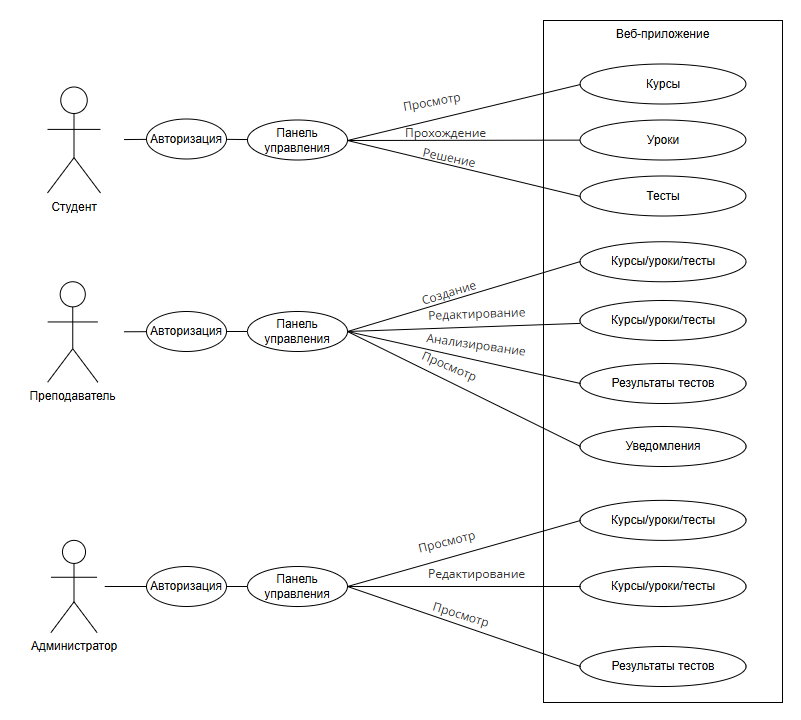
\includegraphics[width=1\linewidth]{UML}}
	\center{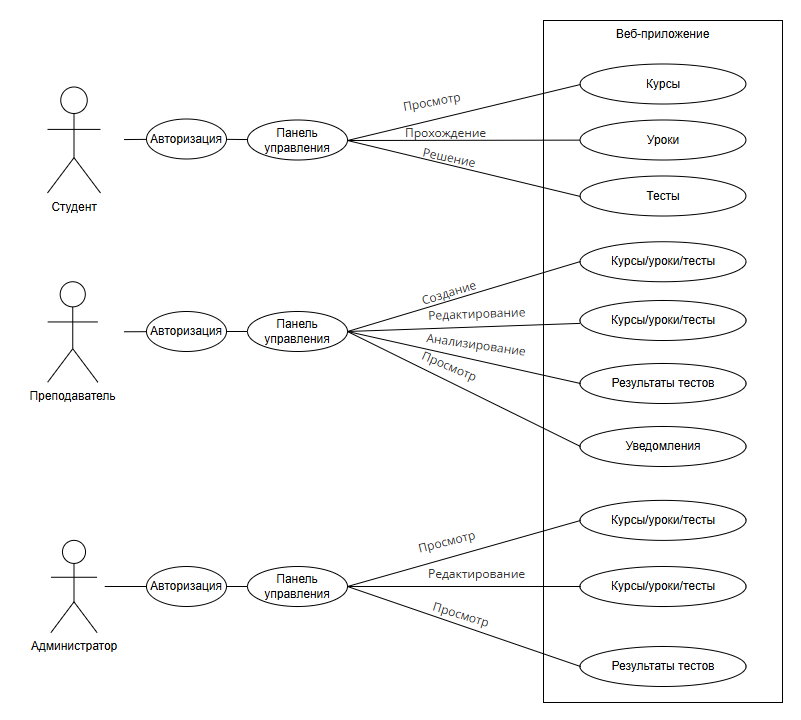
\includegraphics[width=1\linewidth]{UML}}
	\center{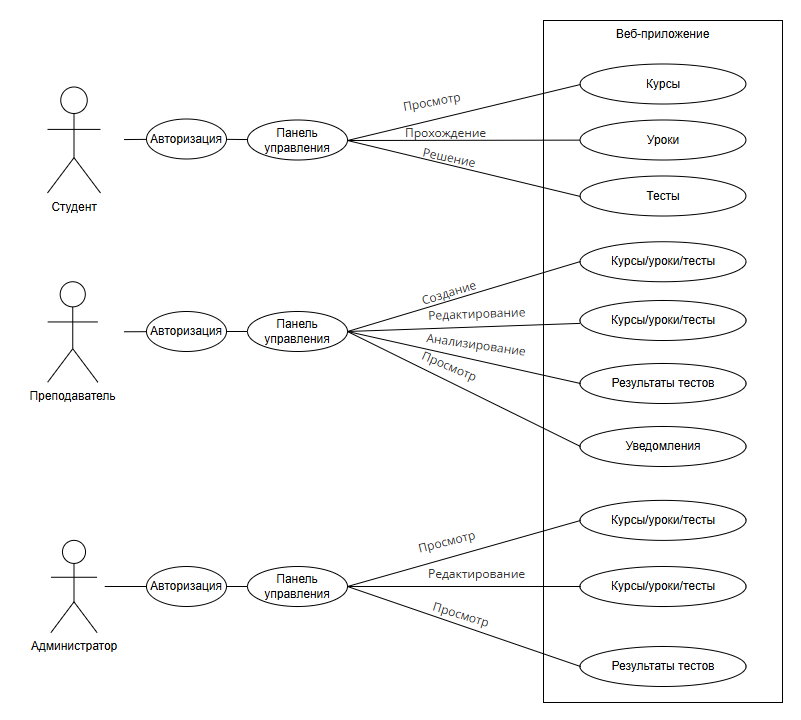
\includegraphics[width=1\linewidth]{UML}}
	\caption{Главная страница обучающей платформы}
	\label{main:image}
\end{figure}

На рисунке \ref{course:image} представлен интерфейс просмотра курса с динамическим отображением уроков и тестов по JavaScript.

\begin{figure}[ht]
	\center{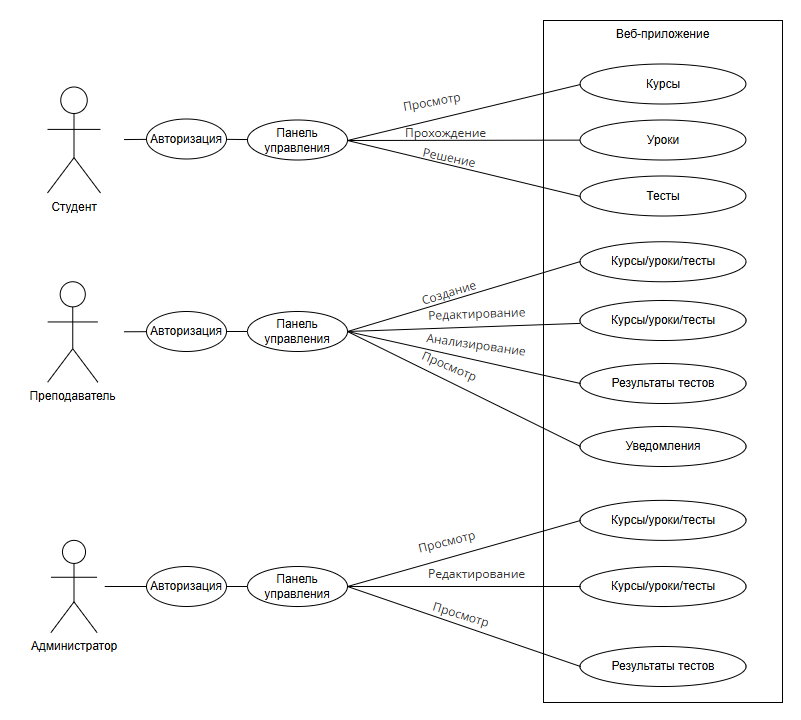
\includegraphics[width=1\linewidth]{UML}}
	\caption{Интерфейс просмотра курса}
	\label{course:image}
\end{figure}

На рисунке \ref{test:image} представлен интерфейс сдачи теста по JavaScript с динамической формой для выбора ответов.

\begin{figure}[ht]
	\center{\includegraphics[width=1\linewidth]{курсы}}
	\caption{Интерфейс сдачи теста}
	\label{test:image}
\end{figure}
   \section*{ЗАКЛЮЧЕНИЕ}
\addcontentsline{toc}{section}{ЗАКЛЮЧЕНИЕ}

Преимущества аддитивных технологий заключается в разнообразии процессов, позволяющих применять их в различных областях производства. Существенным ограничением же является и экономическая составляющая, которая не позволит внедрить аддитивное производство повсеместно.
  
Компании, видя, как развиваются информационные технологии, пытаются использовать их выгодно для своего бизнеса, запуская свой сайт для того, чтобы заявить о своем существовании, проинформировать потенциального клиента об услугах или продуктах, которые предоставляет. 
Для продвижения компании «Русатом – Аддитивные технологии» был разработан веб-сайт на основе системы «1С-Битрикс: Управление сайтом».

Основные результаты работы:

\begin{enumerate}
\item Проведен анализ предметной области. Выявлена необходимость использовать 1С-Битрикс.
\item Разработана концептуальная модель web-сайта. Разработана модель данных системы. Определены требования к системе.
\item Осуществлено проектирование web-сайта. Разработана архитектура серверной части. Разработан пользовательский интерфейс web-сайта.
\item Реализован и протестирован web-сайт. Проведено модульное и системное тестирование.
\end{enumerate}

Все требования, объявленные в техническом задании, были полностью реализованы, все задачи, поставленные в начале разработки проекта, были также решены.

Готовый рабочий проект представлен адаптивной версткой сайта. Сайт находится в публичном доступе, поскольку опубликован в сети Интернет.  

}\fi
\addcontentsline{toc}{section}{СПИСОК ИСПОЛЬЗОВАННЫХ ИСТОЧНИКОВ}

\begin{thebibliography}{9}

    \bibitem{javascript5} Бейли, Р. Методика преподавания программирования иностранным студентам / Р. Бейли. – Москва: Лань, 2021. – 210 с. – ISBN 978-5-8114-5678-9. – Текст~: непосредственный.
    
    \bibitem{javascript1} Браун, И. Изучаем JavaScript: руководство по созданию современных веб-сайтов / И. Браун. – Москва: Эксмо, 2022. – 480 с. – ISBN 978-5-04-123456-7. – Текст~: непосредственный.
    
    \bibitem{css1} Веру, Л. CSS-секреты. 47 советов по улучшению веб-интерфейсов / Л. Веру. – Санкт-Петербург: Питер, 2017. – 368 с. – ISBN 978-5-496-02699-4. – Текст~: непосредственный.
    
    \bibitem{html1}	Голдстайн, А. HTML5 и CSS3 для всех / А. Голдстайн, Л. Лазарис, Э. Уэйл. – Москва~: Вильямс, 2012. – 368 с. – ISBN 978-5-699-57580-0. – Текст~: непосредственный.
    
    \bibitem{htmlcss} Дэкетт, Д. HTML и CSS. Разработка и создание веб-сайтов / Д. Дэкетт. – Москва: Эксмо, 2014. – 480 с. – ISBN 978-5-699-64193-2. – Текст~: непосредственный.
	
    \bibitem{javascript2} Кантор, Д. JavaScript для начинающих: от основ до веб-приложений / Д. Кантор. – Санкт-Петербург: Питер, 2023. – 360 с. – ISBN 978-5-4461-2345-2. – Текст~: непосредственный.
    
    \bibitem{sqlite} Кинг, Д. SQLite. Руководство разработчика / Д. Кинг. – Москва: Вильямс, 2021. – 256 с. – ISBN 978-5-8459-1876-3. – Текст~: непосредственный.
    
    \bibitem{js3} Кларк, А. Технологии адаптивного обучения в IT-образовании / А. Кларк. – Санкт-Петербург: БХВ, 2022. – 180 с. – ISBN 978-5-9775-0987-6. – Текст~: непосредственный.
    
    \bibitem{javascript3} Макфарланд, Д. JavaScript и jQuery: интерактивная фронтенд-разработка / Д. Макфарланд. – Москва: Диалектика, 2021. – 512 с. – ISBN 978-5-907203-45-6. – Текст: непосредственный.  

    \bibitem{python1} Матей, Н. Python. К вершинам мастерства / Н. Матей. – Санкт-Петербург: Питер, 2022. – 432 с. – ISBN 978-5-4461-0926-5. – Текст~: непосредственный.
	
	\bibitem{python} Петров, И. П. Python для веб-разработки: от основ до продвинутых техник / И. П. Петров. – Санкт-Петербург: Питер, 2024. – 416 с. – ISBN 978-5-4461-1789-5. – Текст~: непосредственный.
	
    \bibitem{javascript4} Симпсон, К. Глубокая работа с JavaScript: замыкания, прототипы, асинхронность / К. Симпсон. – Санкт-Петербург: Питер, 2022. – 288 с. – ISBN 978-5-4461-1987-5. – Текст~: непосредственный.  
	
	\bibitem{html2}	Титтел, Э. HTML5 и CSS3 для чайников / Э. Титтел, К. Минник. – Москва~: Вильямс, 2016 – 400 с. – ISBN 978-1-118-65720-1. – Текст~: непосредственный.
	
	\bibitem{django}	Холл, Б. Django. Разработка веб-приложений / Б. Холл.– Москва: ДМК Пресс, 2023.– 512 с. – ISBN 978-5-97060-789-0.– Текст~: непосредственный.
	
    \bibitem{css2} Юэнс, В. CSS. Карманный справочник / В. Юэнс. – Москва: Символ-Плюс, 2020. – 272 с. – ISBN 978-5-93286-362-0. – Текст~: непосредственный.


\end{thebibliography}

\ifВКР{%\appendix{Представление графического материала}

Графический материал, выполненный на отдельных листах,
изображен на рисунках А.1--А.\arabic{числоПлакатов}.
\setcounter{числоПлакатов}{0}

\renewcommand{\thefigure}{А.\arabic{figure}} % шаблон номера для плакатов

\begin{landscape}

\begin{плакат}
    \includegraphics[width=0.82\linewidth]{бд}
    \заголовок{Сведения о ВКРБ}
    \label{pl1:image}      
\end{плакат}

\begin{плакат}
    \includegraphics[width=0.82\linewidth]{бд}
    \заголовок{Цель и задачи разработки}
    \label{pl2:image}      
\end{плакат}

\begin{плакат}
    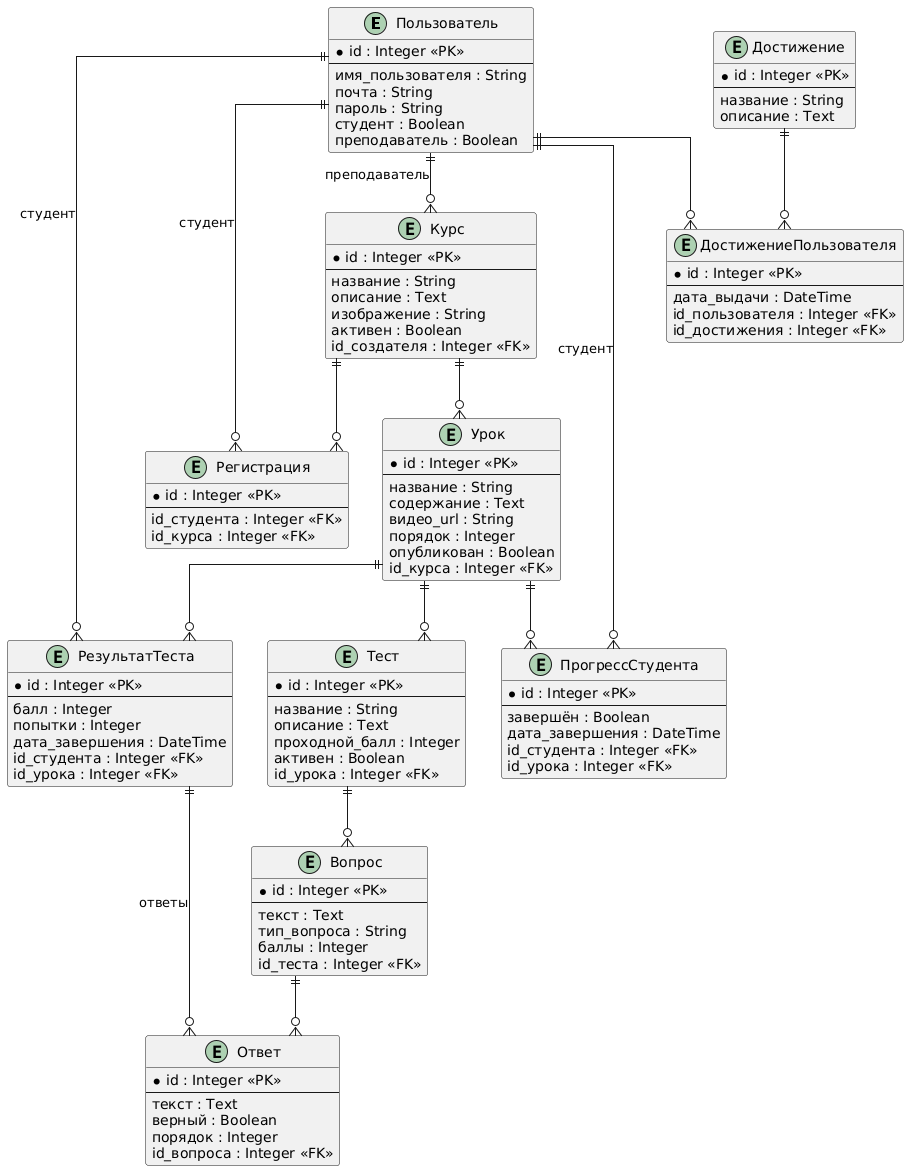
\includegraphics[width=0.6\linewidth]{концептуальная}
    \заголовок{Концептуальная модель сайта}
    \label{pl3:image}      
\end{плакат}

\begin{плакат}
    \includegraphics[width=0.82\linewidth]{бд}
    \заголовок{Еще плакат}
    \label{pl4:image}      
\end{плакат}

\end{landscape}
}\fi
\ifПрактика{}\else{\appendix{Фрагменты исходного кода программы}

views.py
\lstinputlisting[language=python, frame=none]{views.py}


\ifВКР{
\newpage
\addcontentsline{toc}{section}{На отдельных листах (CD-RW в прикрепленном конверте)}
\noindent
\begin{tabular}{p{5.8cm}C{4.8cm}C{4.8cm}}
   Автор ВКР & \lhrulefill{\fill} & \fillcenter\Автор \\
            \setarstrut{\footnotesize}
           & \footnotesize{(подпись, дата)} & \\
            \restorearstrut
   Руководитель ВКР & \lhrulefill{\fill} & \fillcenter\Руководитель \\
            \setarstrut{\footnotesize}
           & \footnotesize{(подпись, дата)} & \\
            \restorearstrut
   Нормоконтроль & \lhrulefill{\fill} & \fillcenter\Нормоконтроль \\
            \setarstrut{\footnotesize}
           & \footnotesize{(подпись, дата)} & \\
            \restorearstrut
\end{tabular}
\vskip 2cm
\begin{center}
\textbf{Место для диска}
\end{center}
}\fi
}\fi
\end{document}
